\chapter{A label-free quantification proteomics pipeline}
\label{chap:pipeline}


\section*{Summary}

A pipeline making use of the set of tools published by the Compomics  and StatOmics groups SearchGUI \cite{Barsnes2018}, PeptideShaker \cite{Vaudel2015}, moFF \cite{Argentini2016} and MSqRob \cite{Goeminne2016} , was developed to support complete label-free protein quantification analyses using the most recent advances in the field with open-source software. The pipeline can be run on Linux computer clusters to perform (I) peptide to spectrum matching against a reference database, (II) quality control and filtering, (III) \ac{MBR} and feature extraction, (IV) protein inference and (V) relative quantification. Its output can be passed to follow-up analyses in R or Python to get a biological interpretation of the results.  A benchmark of its performance was accomplished using the proteome benchmark dataset published in \cite{Cox2014}. The results exhibited an accuracy similar to those achieved by the MaxQuant \cite{Cox2014} software, excepting a bias produced by the sample fractionation of this dataset.


\section{Introduction}

\subsection{Background}

\begin{figure}[!h]
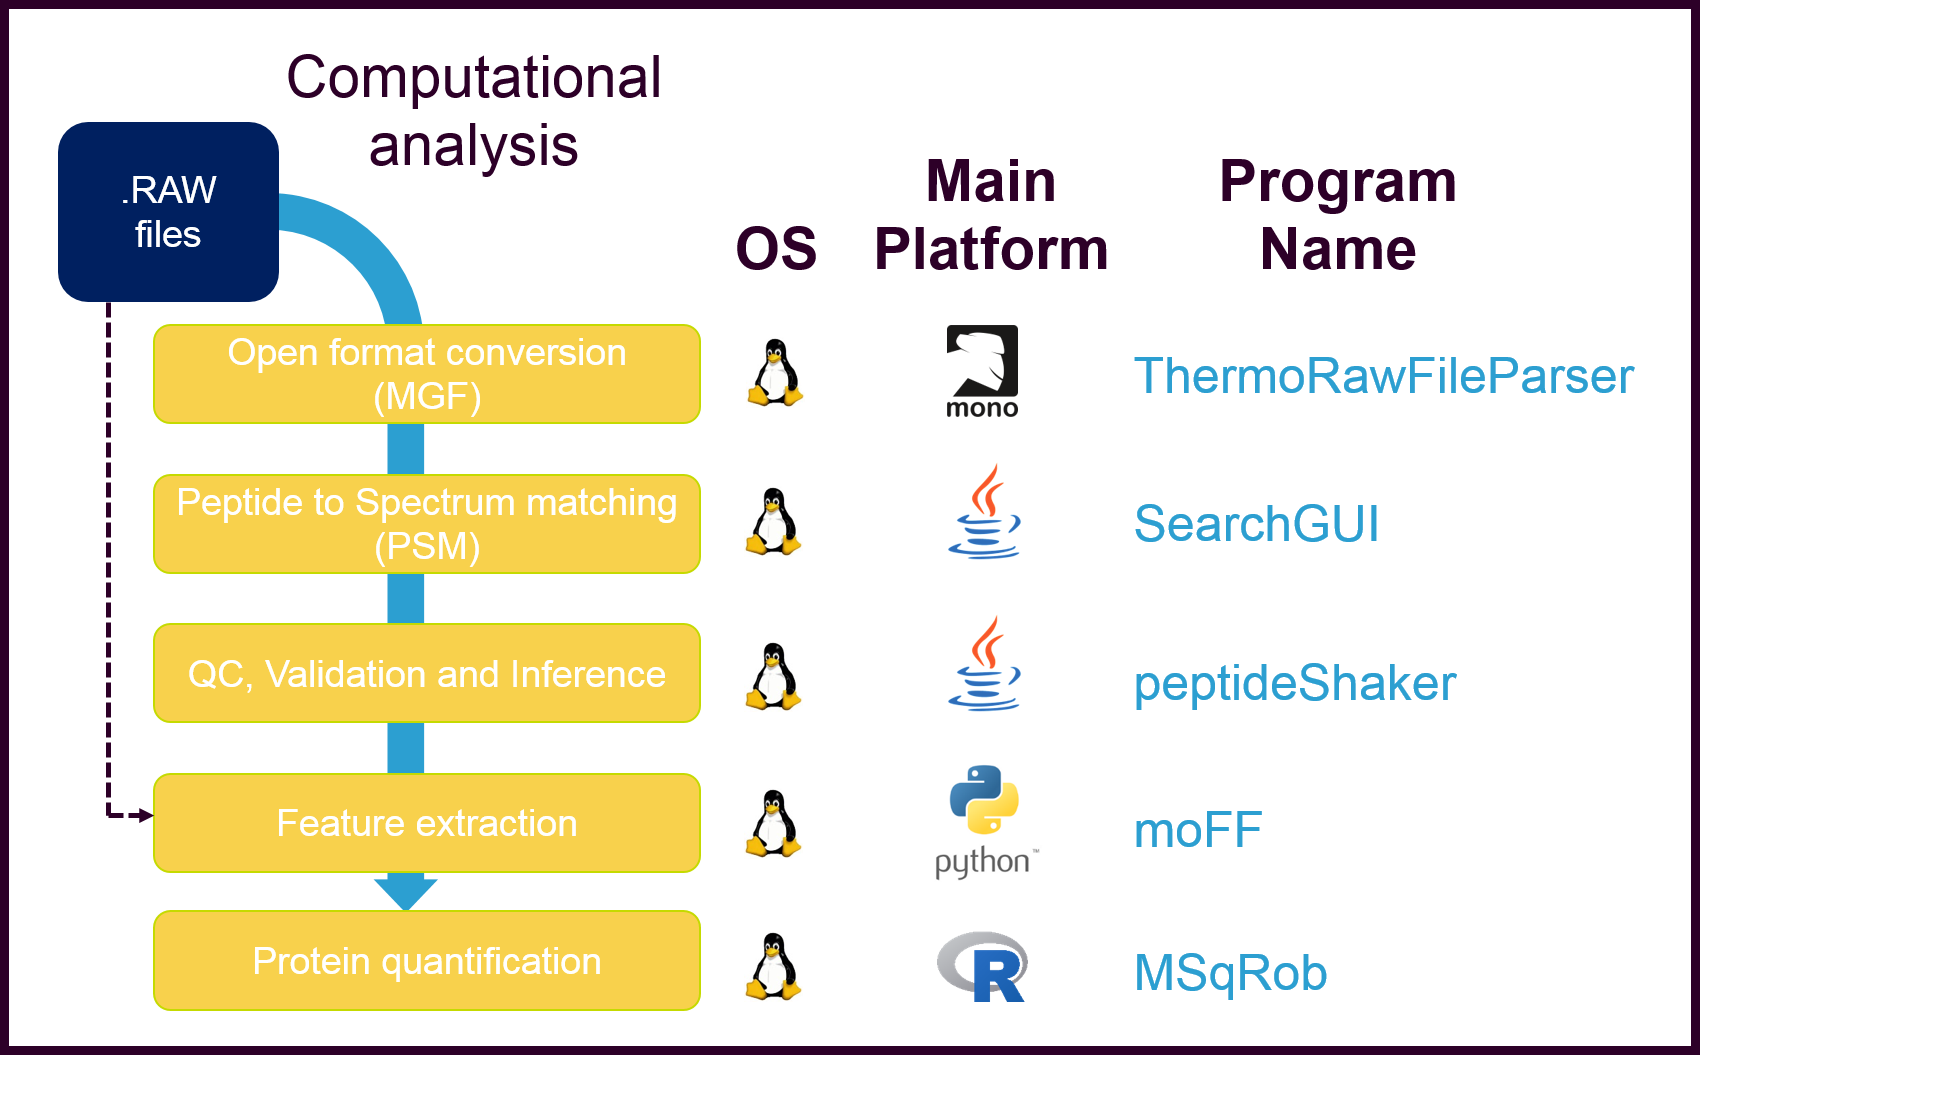
\includegraphics[width=\textwidth]{pipeline}
\mycaption[Schema of the presented pipeline]{First, .RAW files produced by the spectrometer are converted to an open format like the Mascot Generic Format (\ac{MGF}). After that, spectra are searched by means of a search engine to perform the PSM step. Thereafter, PSMs are validated and the most likely set proteins is inferred. If quantative information is to be extracted, a quantification step attempting to estimate protein quantities is executed. The biological interpretation of the pipeline results can be achieved by interacting with public databases using R/Bioconductor or Python thanks to their open format.}
\label{fig:pipeline}
\end{figure}


Several proteomics pipelines are available on the internet under different licensing conditions. Many are released as closed-source commercial software, where information on how the program works is kept from the user. This is a serious drawback as it hinders the study of the implemented models and its customisation. Open-source, free alternatives, like the Trans Proteomic Pipeline (\ac{TPP}) \cite{Deutsch2011} or openMS \cite{Sturm2008} are nevertheless available for the community, but they either lack good documentation, good broad base or format exchangeability. MaxQuant, a freeware but closed-source, monolithic proteomics analysis suite \cite{Cox2008}, is developed for Windows and has only very recently been ported to Linux \cite{Sinitcyn2018}. Nevertheless has been extremely successfully adopted by the scientific community due to its ease of use and comprehensive pipeline.

\subsection{Goals}

The development of a pipeline attempting to achieve the following goals will be described in this chapter.

\begin{enumerate}

\item Fully command line, documented and Linux-supported interface for easy automation and scalability.
\item Open-source for easy customisation and innovation of analyses.
\item Free-licensed and cost-free, so anybody with the knowledge can run it, democratizing the analyses.
\end{enumerate}

\section{Materials and Methods}

\subsection{Data generation and loading}

The proteome benchmark dataset from \cite{Cox2014} was reanalysed starting at the output RAW files available at the PRIDE repository \footnote{\href{https://www.ebi.ac.uk/pride/archive/projects/PXD000279}{https://www.ebi.ac.uk/pride/archive/projects/PXD000279}}. Briefly, the \textit{Homo sapiens} and \textit{E. coli (strain K12)} proteomes were mixed in 1:1 (condition L) and 1:3 (condition H) proportions, with 3 replicates for each combination. Moreover, each of the 3 replicates of the 2 conditions was analysed over 24 fractions. This experimental setting thus generated a total of $2 \times 3 \times 24=144$ RAW files. One file was missing in the repository. The ThermoRawFileParser \footnote{\href{https://github.com/compomics/ThermoRawFileParser}{https://github.com/compomics/ThermoRawFileParser}} program was used to convert RAW files to the MGF open format.

The MQ+LFQ pipeline results were obtained starting at the Supplemental table 1 from the MaxLFQ paper supplemental data \footnote{\href{http://www.mcponline.org/content/13/9/2513/suppl/DC1}{http://www.mcponline.org/content/13/9/2513/suppl/DC1}} \cite{Cox2014}, which is available as an excel file. The results of the MQ+Rob pipeline employed the Levenberg-Marquandt minimised peptide intensities stored in the peptides.txt file contained in the spectraHeLaEColi.zip in the supplemental data.

%\href{http://www.mcponline.org/content/suppl/2014/06/17/M113.031591.DC1/mcp.M113.031591-1.xlsx}{http://www.mcponline.org/content/suppl/2014/06/17/M113.031591.DC1/mcp.M113.031591-1.xlsx}.

\subsection{Decoy database preparation and search}
\label{subsec:database_preparation}

The spectra saved in the MGF files obtained in the previous step were passed to the MS-GF+ search engine \cite{Kim2014} by means of the SearchGUI \texttt{SearchCLI} tool \cite{Barsnes2018} utility. The search parameters were set using the \texttt{IdentificationParametersCLI}. In order to account for potential post-translational modifications, the search was conducted allowing for the following variable modifications: oxidation of M and deamidation of N and Q. Moreover, C carbamidomethylation was set as fixed modification. The enzyme was set to semispecific Trypsin, allowing for a non-tryptic cleavage on any side of the peptide. Up to two missed cleavages were allowed. The precursor tolerance was 10 ppm and the fragment tolerance 0.5 Da. 


The target database was created by combining the Uniprot proteomes for \textit{E. coli (strain K12)} (UP000000625) and \textit{Homo sapiens} (UP000005640), downloaded in June 2018. The decoy database was created using the \texttt{FastaCLI} utility in SearchGUI by reversing all sequences in the target.

\subsection{Quality control and validation}

The SearchGUI results were filtered using the default built-in checks available in the PeptideShaker utility \texttt{PeptideShakerCLI} \cite{Vaudel2015} \footnote{\href{https://github.com/compomics/peptide-shaker/issues/300}{https://github.com/compomics/peptide-shaker/issues/300}}. By default, the FDR was set to 1\%. PEP and confidence statistics were computed using the PeptideShaker built-in algorithms. Output was extracted via the Default PSM report txt file, available in the \texttt{ReportCLI} utility.


\subsection{Data refinement}

The moFF command line utility \cite{Argentini2016} was applied to perform (I) match-between-runs and (II) extract MS1 apex intensity of each peak cluster. This required passing the original RAW files, together with the Default PSM report from PeptideShaker. Output was exported to a peptide summary file, containing  one row per peptide and for every peptide, the detected apex intensity in each sample.

\subsection{Quantification}

Relative quantification was performed using the MSqRob utility by passing the peptide summary file from moFF. Prior to quantification, the data was preprocessed using the \texttt{preprocess\_MSnSet()} function. In a nutshell, (I) MS1 apex intensities were $log_2$ transformed, (II) quantile normalized, (III) peptides belonging to protein groups that contained one or more proteins that were also present in a smaller protein group were discarded \cite{Goeminne2016}, and (IV) protein groups with only 1 peptide were dropped.

Once preprocessing is done, a ridge regression model with Huber weights and empirical Bayes estimation of protein variance, implemented in the MSqRob package \cite{Goeminne2016}, was fit to every protein individually. The peptide and fraction effects were considered random, while the condition was treated as a fixed effect. The significance of the treatment effect differences was assessed through a Student\textquotesingle s T test, implemented in the \texttt{test.contrast()} function. Only protein groups that could be unambiguously mapped to one of the organisms were considered for the analysis.

Quantification in the MQ+LFQ pipeline was executed using the LFQ intensity columns stored in the supplemental data file. Intensities were log2 transformed and averaged. The difference between conditions H and L was taken as estimate of the log2FC. Significance was evaluated by means of the two-tailed Welch Two Sample t-test implemented in the \texttt{t.test()} function in R. P-values were corrected using the FDR method implemented in the \texttt{p.adjust()} function in R.


\subsection{Code implementation}

\section{Results}

\subsection{Evaluation of the PSM step}

The preprocessing of the RAW files produced by the mass spectrometer into the MGF open format enabled searchGUI to dispose of the registered spectra. PeptideShaker quality control and filtering capabilities (see figure \ref{figure:qc_validation}) carried out the required search results validation. As expected, matches to the target and decoy exhibited similar score distributions at low score values, while a divergence is observed at higher score values. Likewise, the m/z error was found to be closer to 0 on validated PSMs than on those which did not pass the 1 \% FDR filter. The application of this filter implied that the FNR (false negative rate) was set to 5 \%, i.e 5 out of every 100 discarded matches were estimated to be true positives.



\begin{figure}[!h]
\centering
\begin{subfigure}{.45\textwidth}
  \centering
  \caption*{A}
  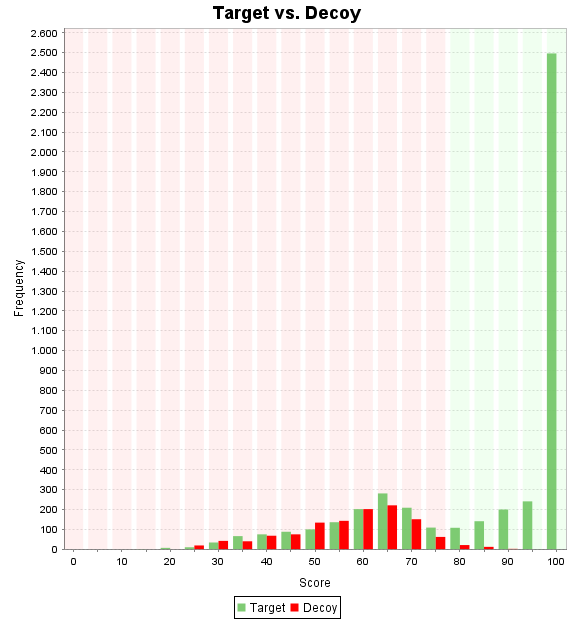
\includegraphics[width=.9\linewidth]{target_vs_decoy}
\end{subfigure}
\begin{subfigure}{.45\textwidth}
  \centering
    \caption*{B}
  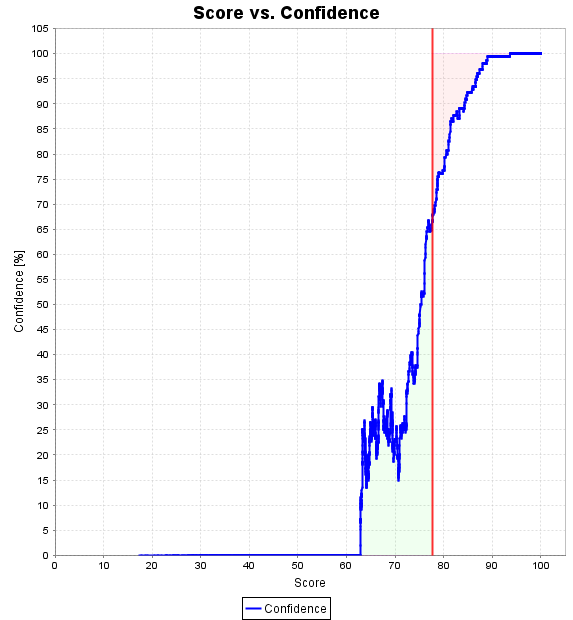
\includegraphics[width=.9\linewidth]{score_vs_confidence}
\end{subfigure}
\bigskip

\begin{subfigure}{.45\textwidth}
  \centering
    \caption*{C}
  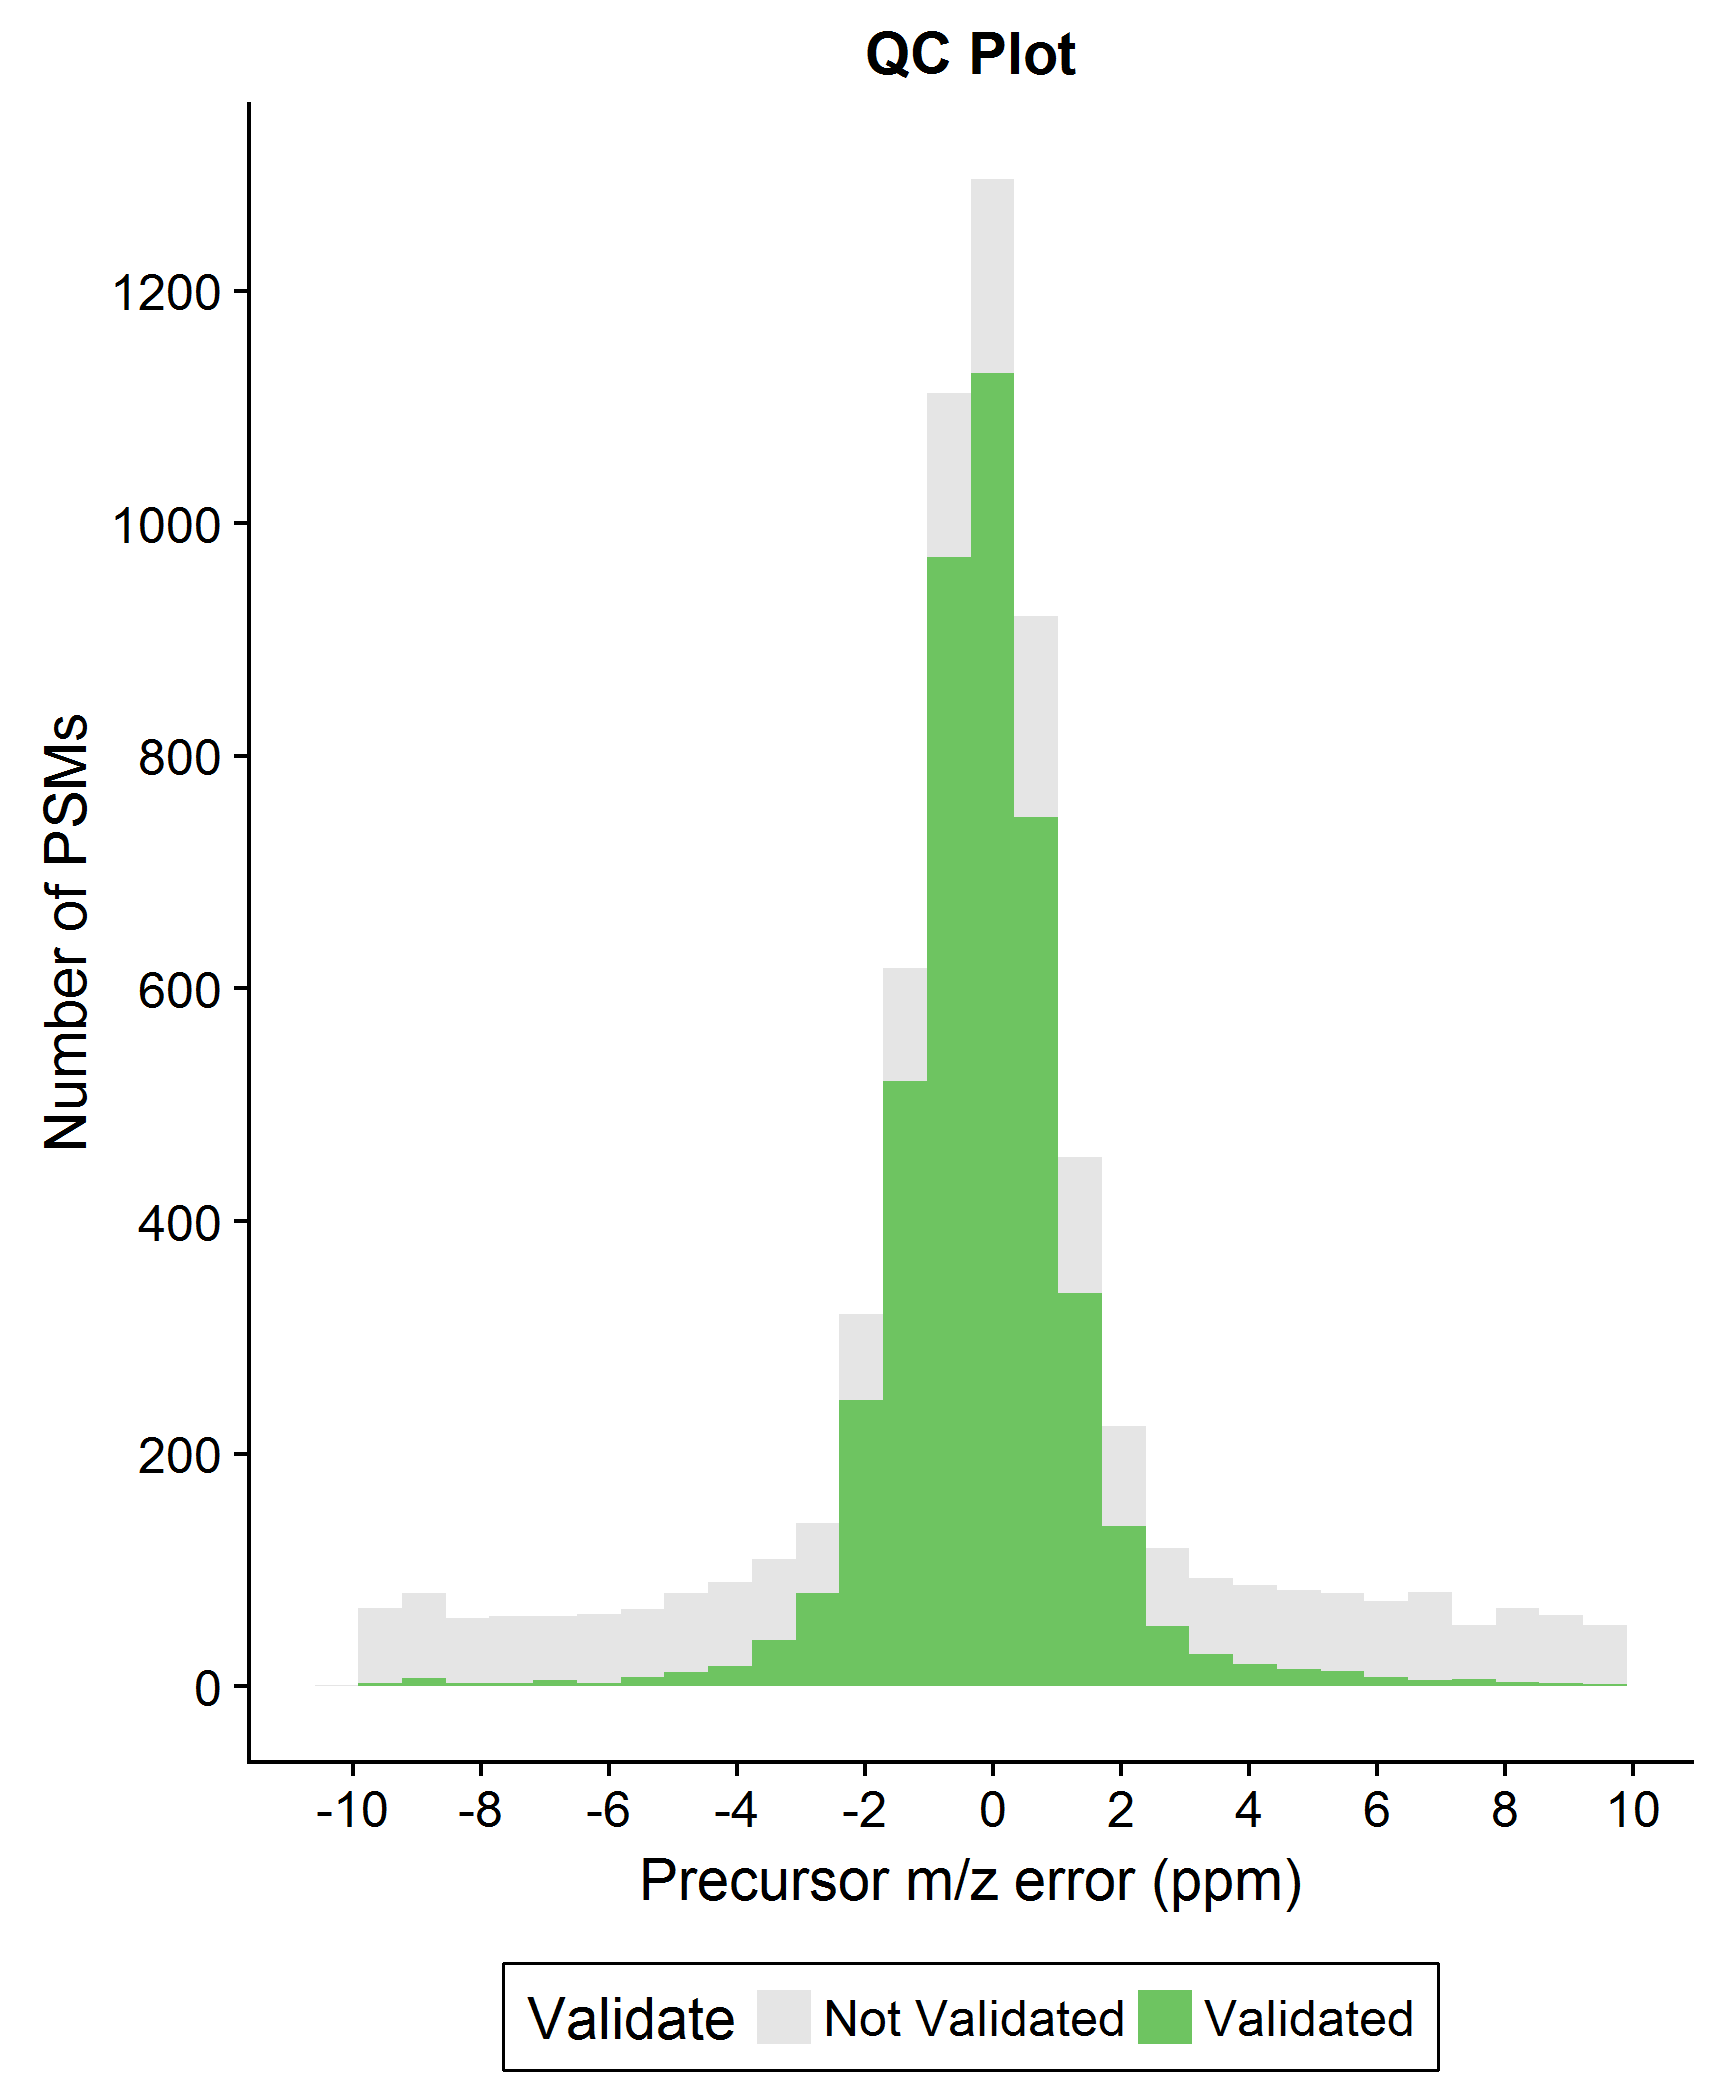
\includegraphics[width=.95\linewidth]{qc}
\end{subfigure}
\begin{subfigure}{.45\textwidth}
  \centering
    \caption*{D}
  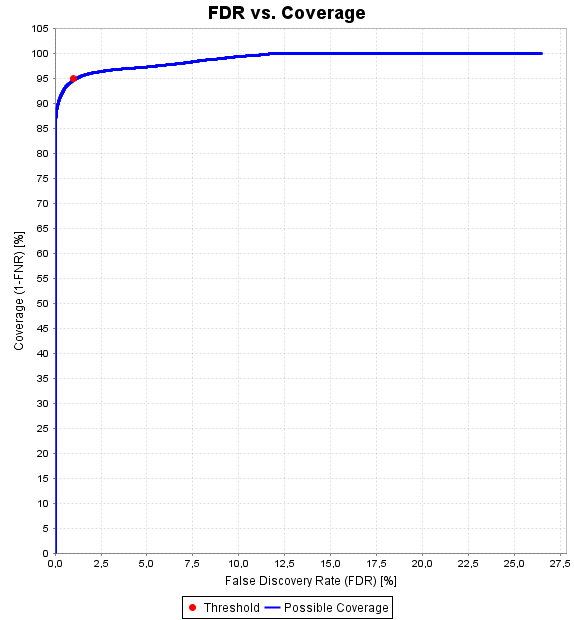
\includegraphics[width=.95\linewidth]{roc}
\end{subfigure}
\mycaption[Quality control and validation of the 13th fraction of the third replicate in condition L]{\textbf{A} Score distribution for matches to the decoy and the target databases. \textbf{B} Evolution of the PSM score with confidence. The implemented cutoff at FDR of 1 \% is displayed with a red vertical line. \textbf{C} Distribution of the difference between the predicted and measured \ac{m/z} values, segregated by validation status. \textbf{D} ROC curve built upon the number of false positives and negatives estimated from the decoy search. The cutoff is displayed as a red dot.}
\label{figure:qc_validation}
\end{figure}

 The 1\% FDR cutoff selected PSMs with a score higher than 78, which translated to a confidence of at least 65\%.


The combination of both programs enabled the identification and validation (matching) of thousands of spectra with high confidence in all samples. However, when compared to the total amount of spectra available, the percentage of matched spectra was on average 37.4\%, with a marked decrease starting at fraction 14 (see figure \ref{fig:match_percent}).

\begin{figure}[!h]
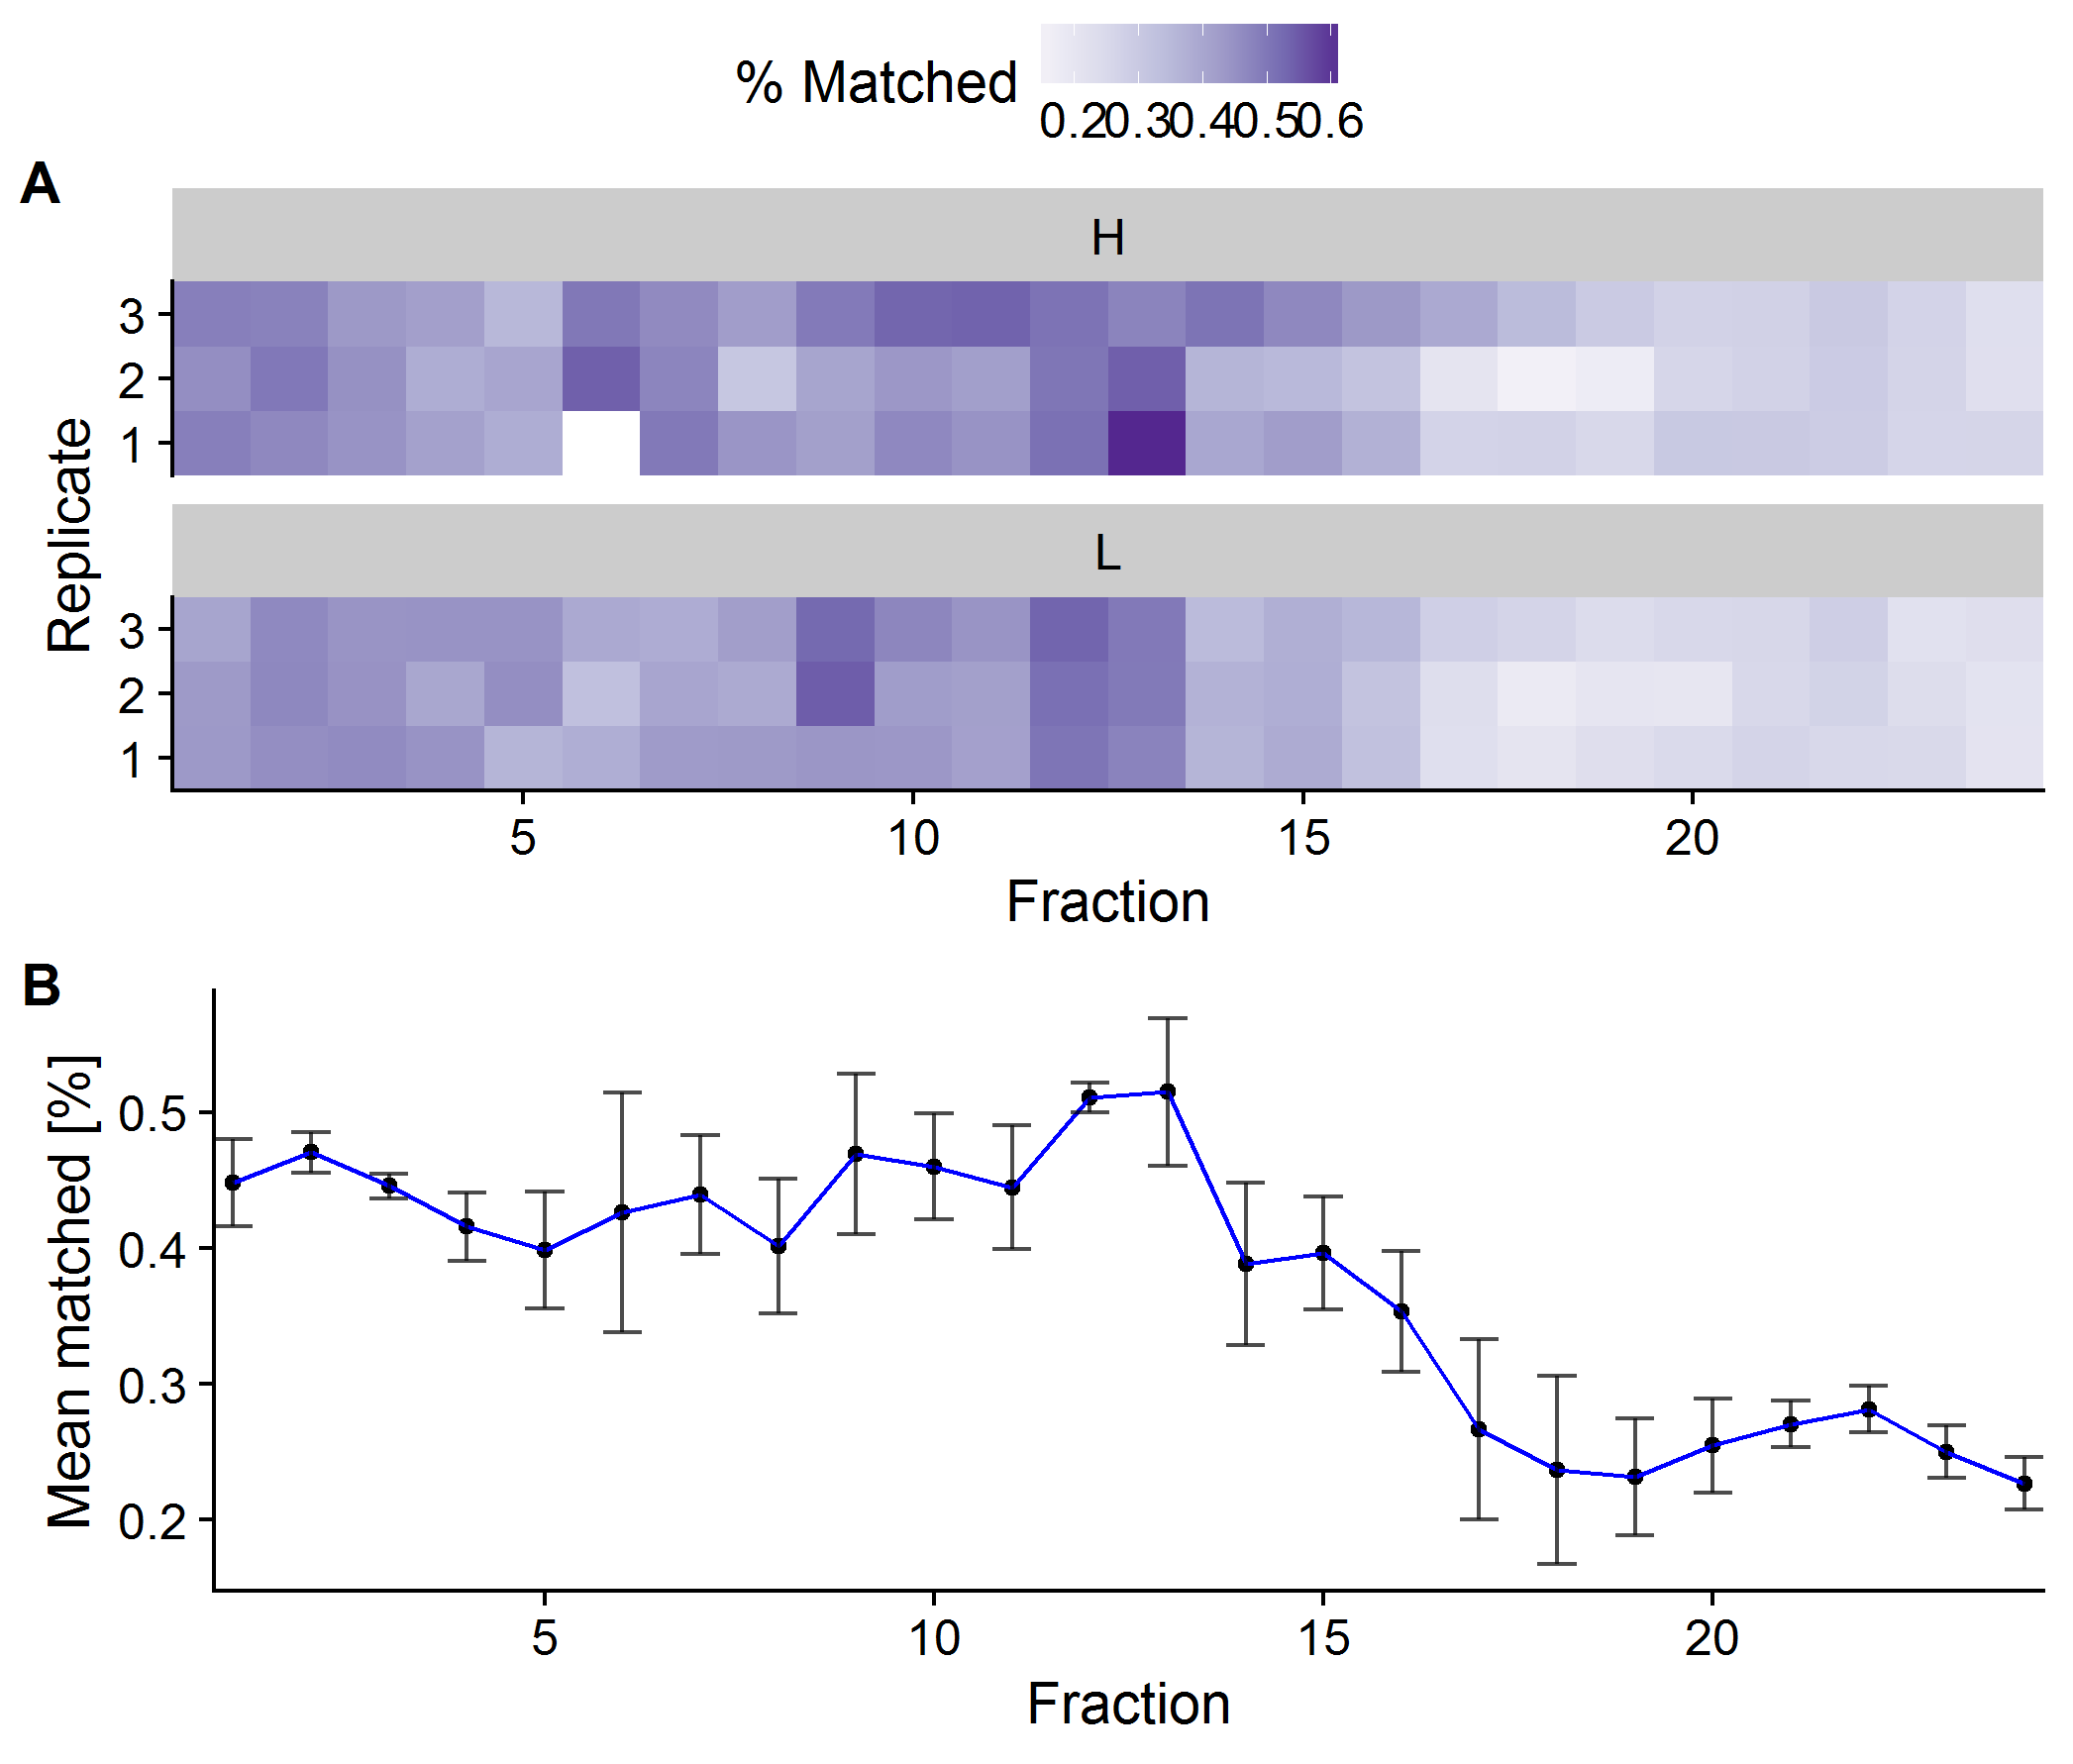
\includegraphics[width=0.8\textwidth]{match_percent}
\mycaption[Percentage of matched spectra in all samples]{The total number of spectra per sample ranged between 5894 and 20249. \textbf{A} Percentages are encoded with a blue palette, the darker, the higher, and viceversa. \textbf{B} The mean for each analysed fraction across conditions and replicates is displayed together with error bars to represent the standard deviation. The sixth fraction of the first replicate in condition H was missing in the PRIDE data repository.}
\label{fig:match_percent}
\end{figure}

\subsection{Protein inference}

\begin{table}[H]
\begin{tabular}{ccccc}
  \toprule
 Total peptides & Unique peptides & Non-unique & Proteins & Protein groups \\ 
  \midrule
 46595 & 27384 & 19211 & 25056 & 10039 \\
 \bottomrule
\end{tabular}
\caption{\textbf{Protein inference results}. The counts of the different molecular entities detected by peptideShaker are displayed.}
\label{tab:protein_inference}
\end{table}

A total of 46595 peptides were inferred to be present in at least one of the fractions (see table \ref{tab:protein_inference}). Of them more than 27 thousand mapped to a unique protein. However, a significant amount mapped to more than one protein. Such peptides are called non-unique peptides. The 25056 detected proteins were grouped into 10039 protein groups. Protein groups are peptide generating entities for which enough data to confirm the presence of at least one of them is available, but not to exactly assess which of them. Thus, protein inference algorithms create them when a does not uniquely map to a protein because it is not possible to distinguish which protein it truly comes from.

Protein groups are very frequent due to several factors. For example, protein isoforms, consisting of protein sequences differing in potentially only one aminoacid, are very difficult to resolve. PeptideShaker executes a smart protein grouping by harnessing the annotation of proteins and classifying protein groups based on how well the annotation backs the protein group.

However, in the present analysis the quality of the protein group was not taken into account, as explained in the Materials and Methods.


\subsection{MBR and apex intensity extraction evaluation}

The match between runs step allowed for increased identifications by transferring successful matches between replicate runs. The results of this process for the 13th fraction of the L condition is shown in figure \ref{fig:mbr}.

\begin{figure}[H]
\centering
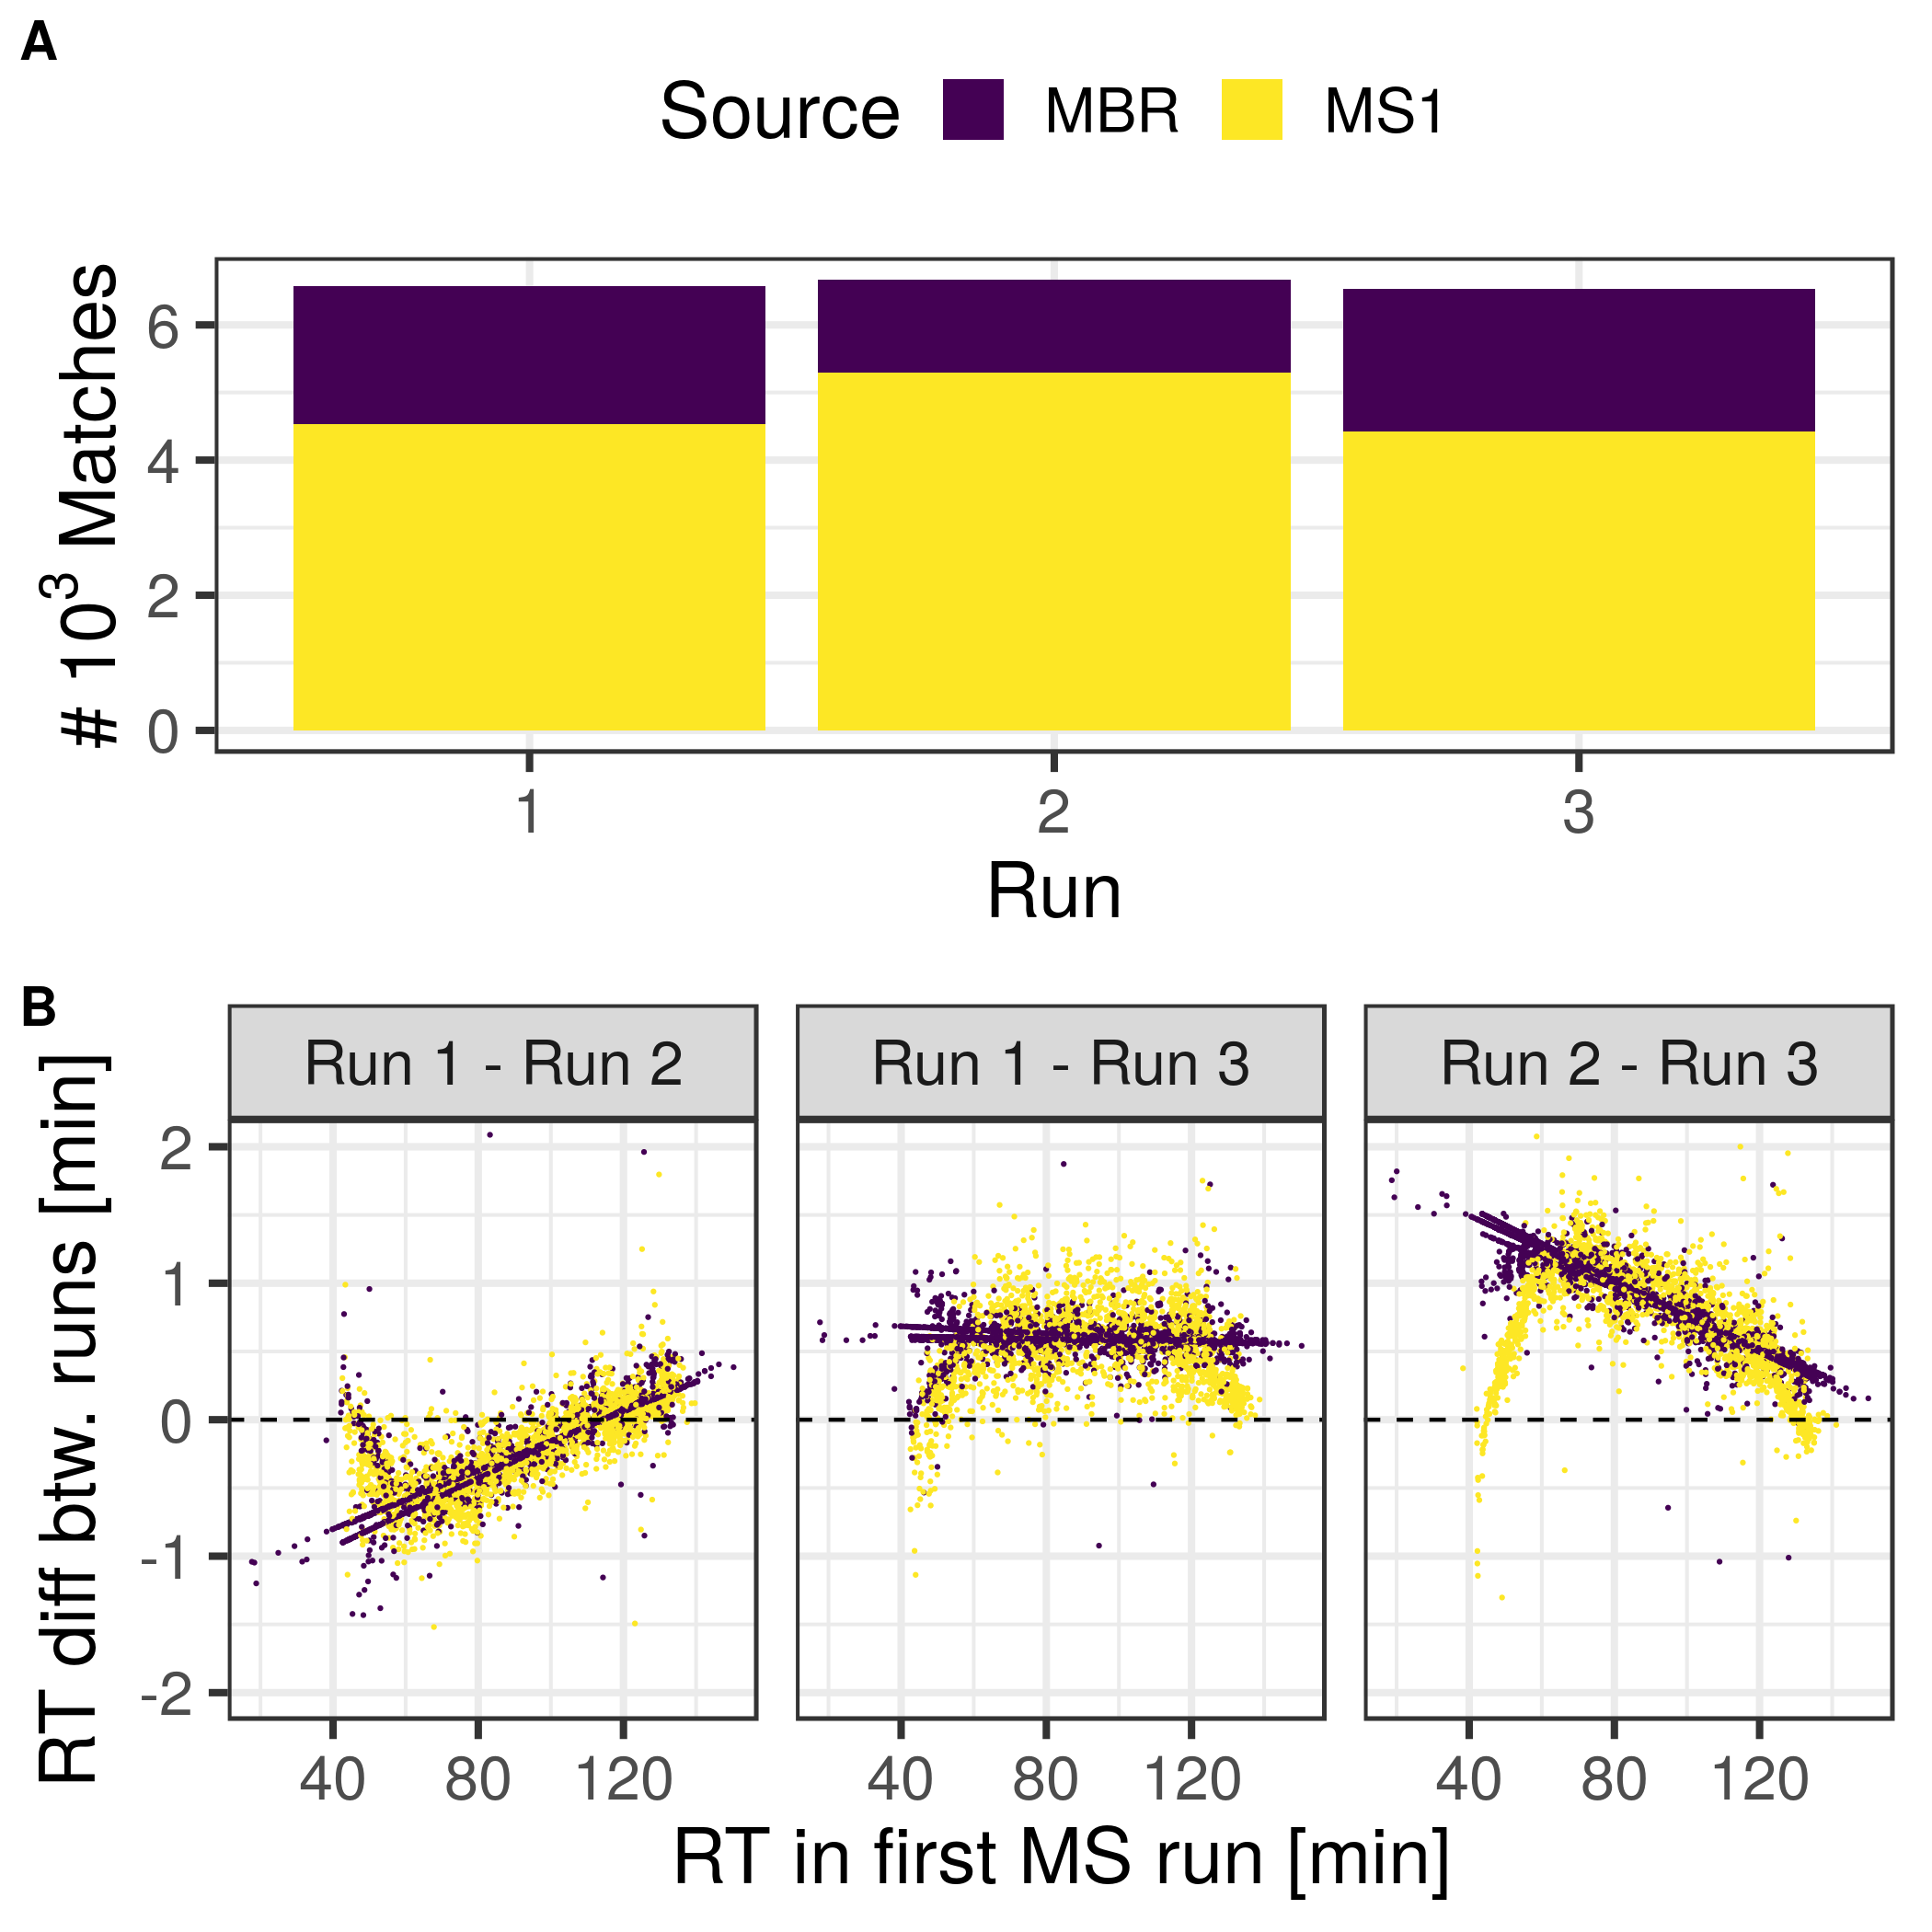
\includegraphics[width=\textwidth]{mbr_combined}
\caption{Match Between Runs with moFF. \textbf{A} Count of identifications on each run segreagated by source. More than 4k spectra were identified and validated by SearchGUI+peptideShaker. In this particular case, hundreds of new identifications were accomplished. \textbf{B} Match visualization. Every dot represents a peptide shared across 2 runs. The coordinate system illustrates its retention time on the first run on the x axis and the difference with the second run on the y axis. The color depicts whether the identification was carried out during the PSM process (MS1), or thanks to a cross-identification achieved by the MBR module (MBR).}
\label{fig:mbr}
\end{figure}

Once as many identifications as possible were gathered, a refinement of the measured MS1 intensity can be implemented to select the apex of every peak cluster, which yields robust intensity measurements for each sample (see figure \ref{fig:apex_intensity}). 

\begin{figure}[H]
\begin{subfigure}{.9\textwidth}
  \centering
    \caption*{A}
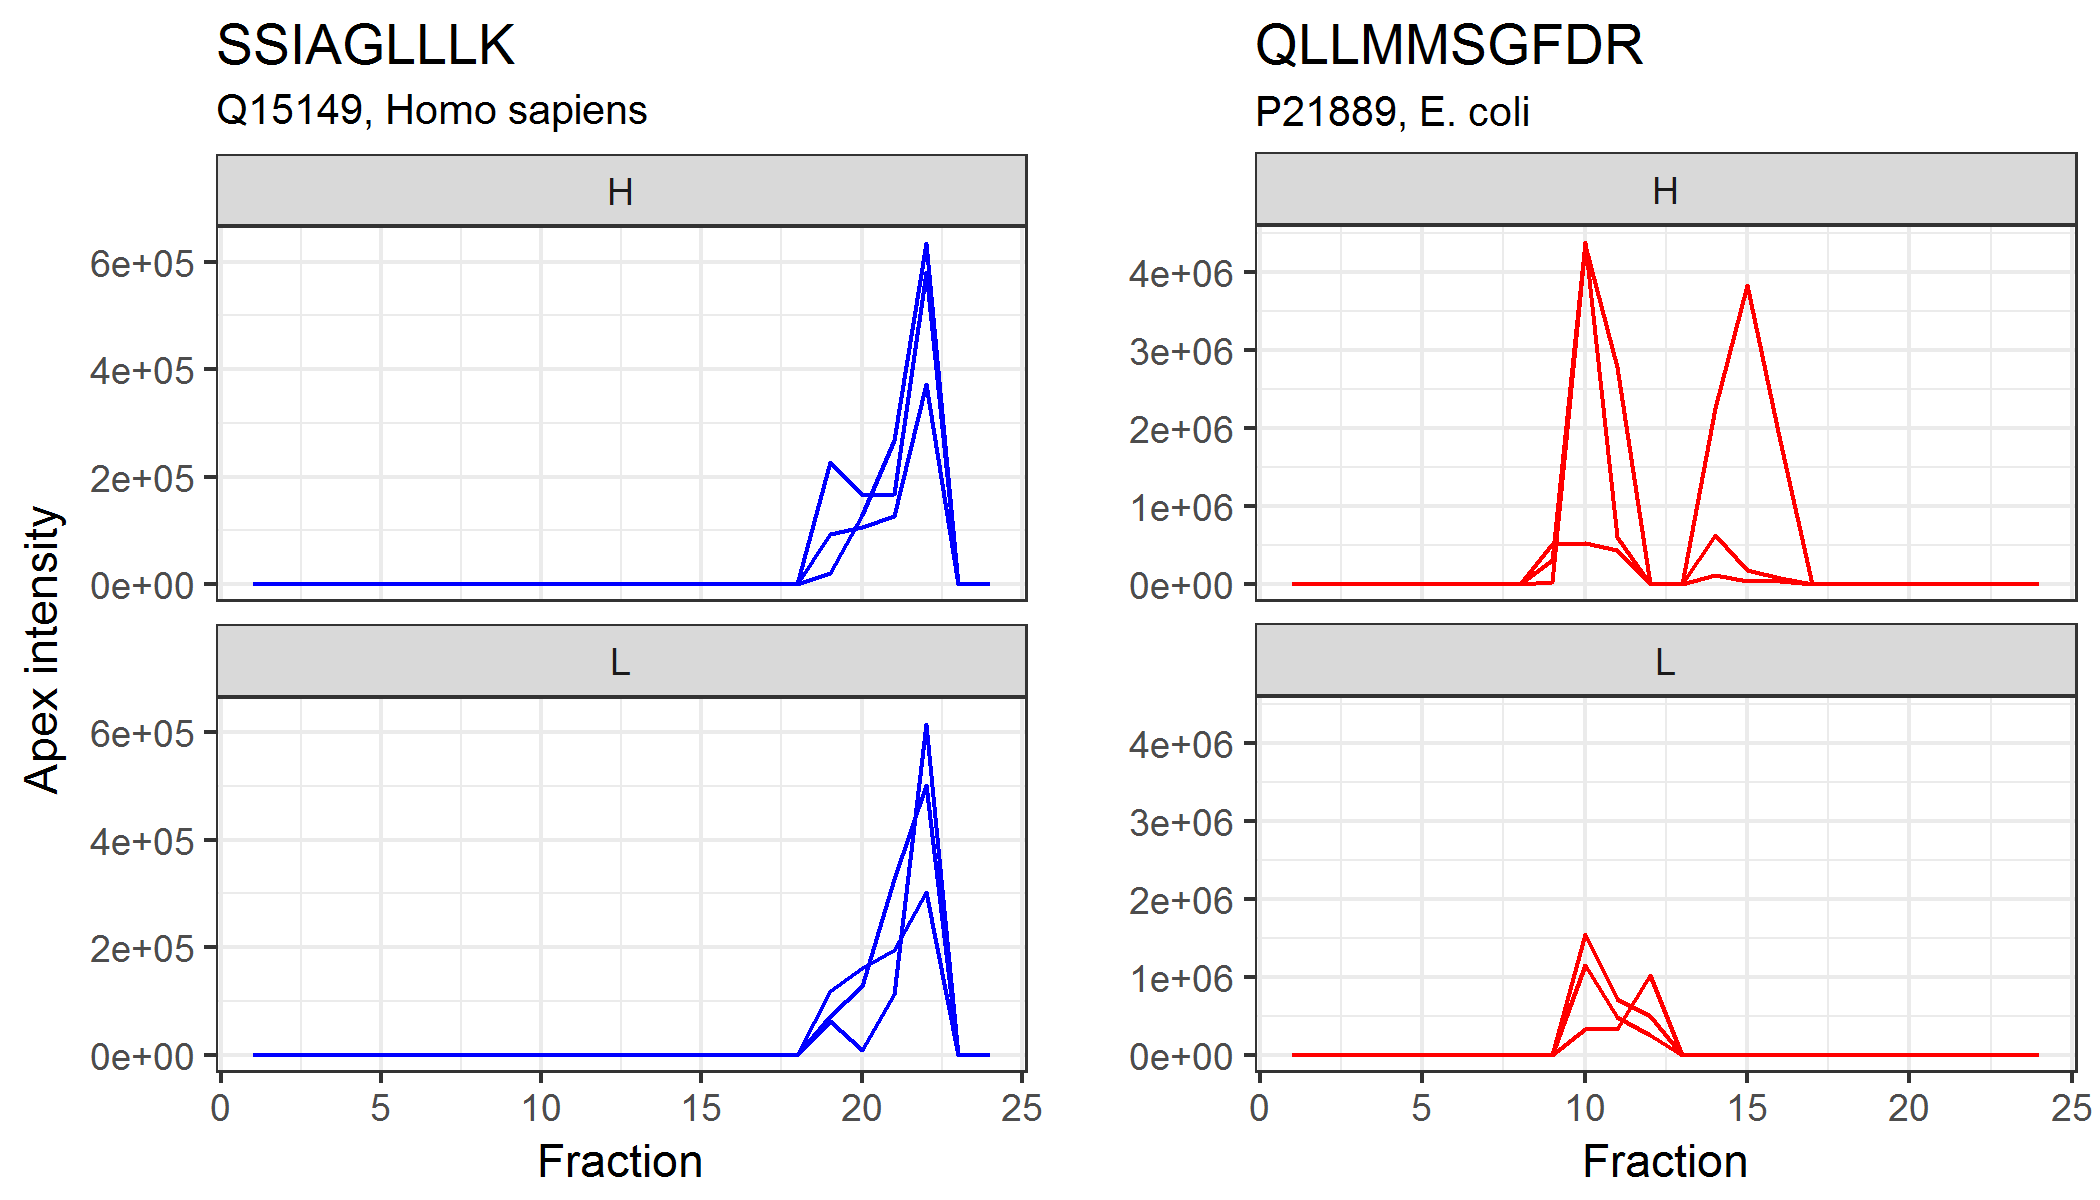
\includegraphics[width=.9\linewidth]{peptide_profile}
\end{subfigure}
\bigskip

\begin{subfigure}{.9\textwidth}
  \centering
    \caption*{B}
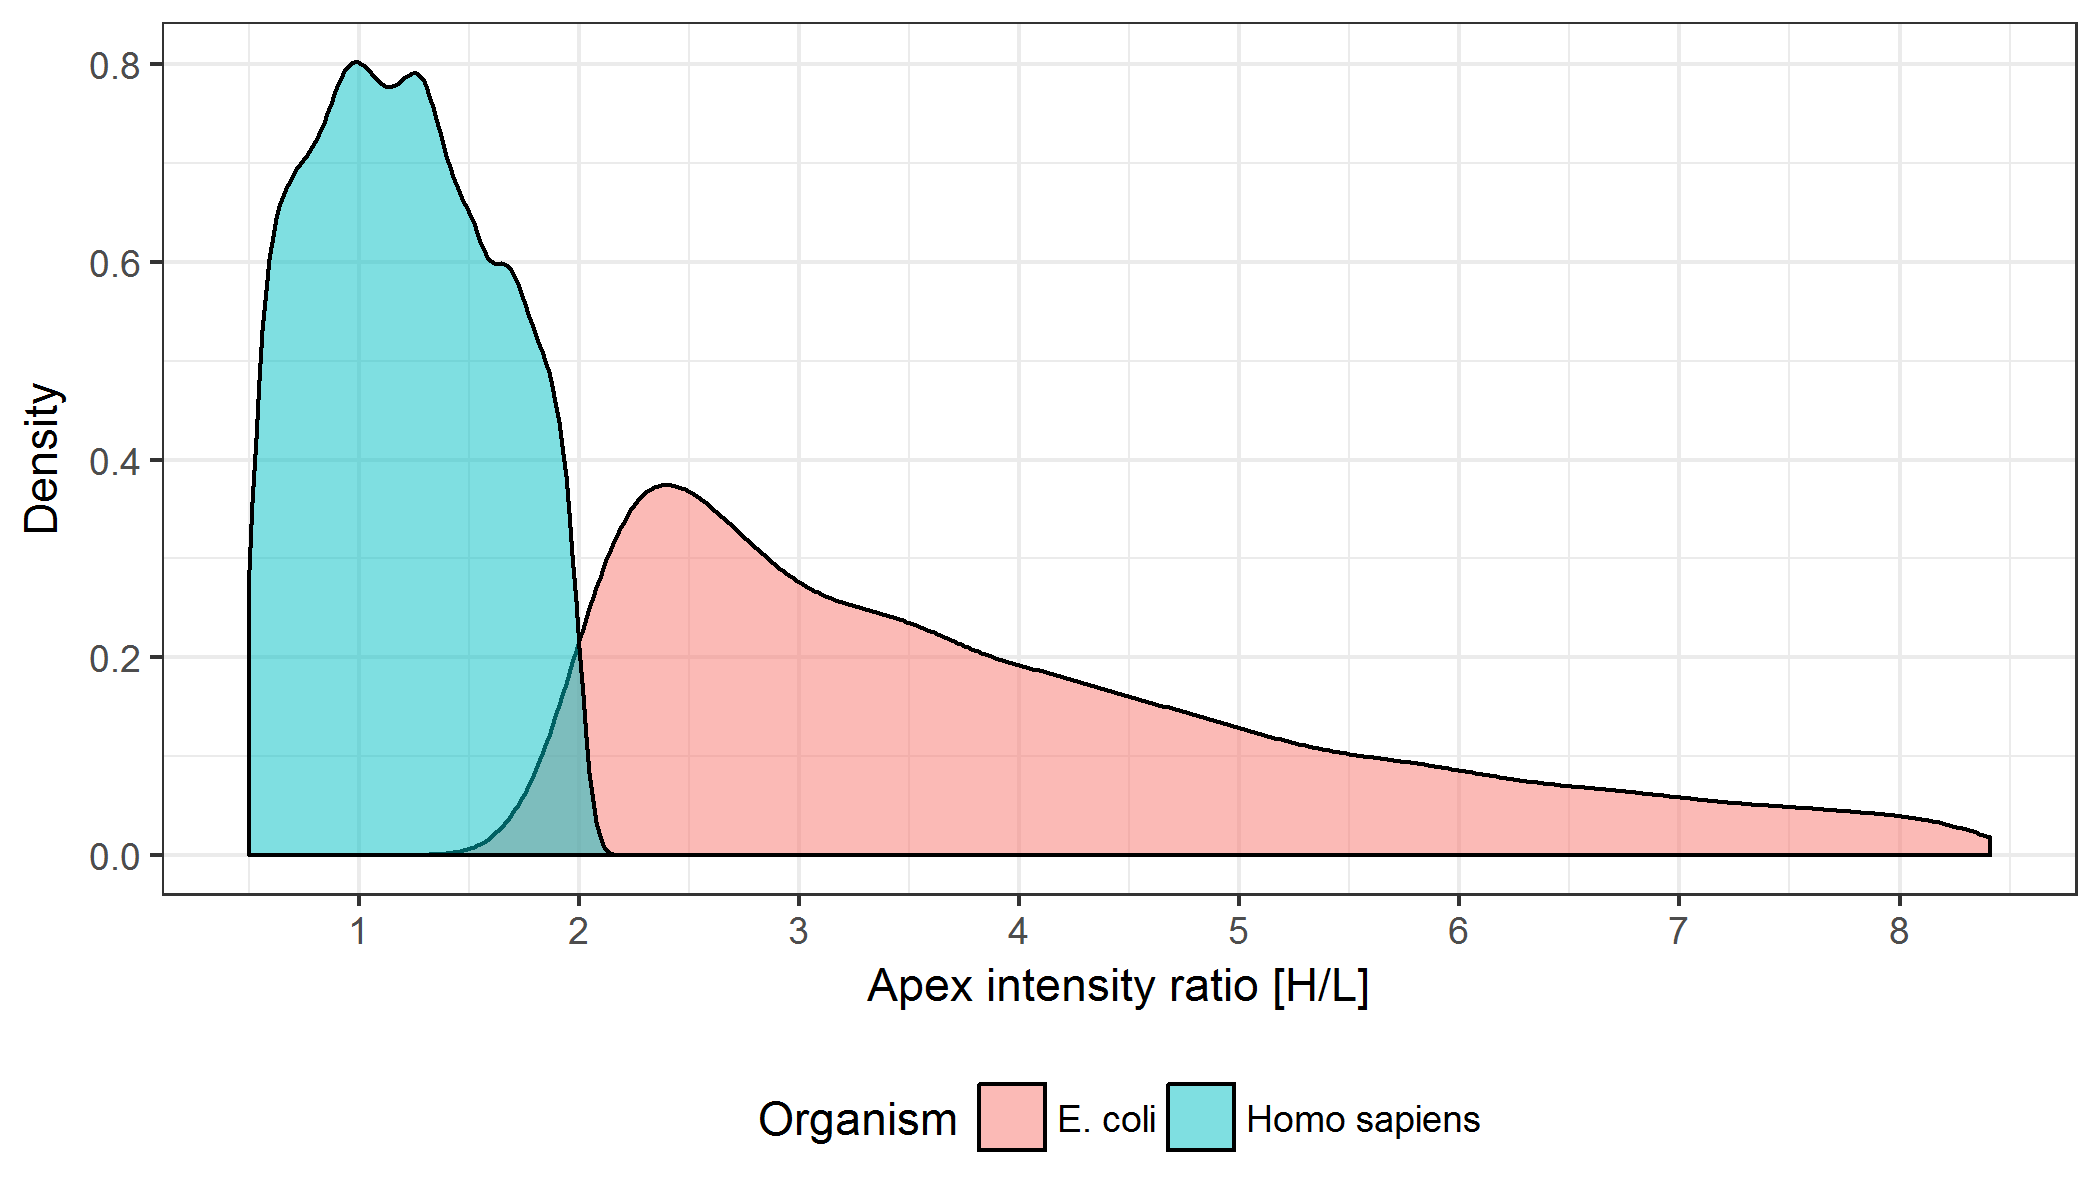
\includegraphics[width=.9\linewidth]{density_ratio}
\end{subfigure}
\caption{\textbf{A} The apex intensity profile across fractions for 2 different peptides, one from \textit{Homo sapiens}, and one from \textit{E. coli}. The figure illustrates the intrinsic intensity variability between technical replicates, particularly in the case of the \textit{E. coli} QLLMMSGFDR peptide, as it was almost non-existent in one of the runs. \textbf{B} The expected pattern of overall similar intensities for the \textit{Homo sapiens} data and 3-fold higher intensities for the \textit{E. coli} data in condition H was observed, confirming an acceptable performance of the protocol.}
\label{fig:apex_intensity}
\end{figure}


\subsection{Quantification benchmark}
\label{subsec:quantification}

The extracted apex MS1 intensities were used as proxy for peptide abundance to estimate protein $\log_2$(ratios), or \textit{log2-fold-changes} (\ac{log2FC}) across condition H and condition L. During quantification, it is important to take into account as many of the effects influencing protein quantification. In this case, besides the different H and L conditions, peptide, run and fraction effects could be distinguished. The MSqRob quantification engine treats effects differently depending on whether or not they are random, or fixed. Fixed effects should have a consistent impact in the ion currents measured in the spectrometer, whereas random effects are truly random and thus unpredictable.

The result of the process was the successful quantification of 5307 protein groups out of 10039 (see table \ref{tab:quantification_table}).

% latex table generated in R 3.4.4 by xtable 1.8-2 package
% Sun Jul 15 18:17:23 2018
\begin{table}[ht]
\centering
\begin{tabular}{llll>{\itshape}l}
  \toprule
 & \ac{log2FC} & qval & Protein & Organism \\ 
  \midrule
1 & -4.76E-01 & 1.42E-24 & P78527 & Homo sapiens \\ 
   \rowcolor[gray]{0.95}2 & 6.80E-01 & 6.75E-24 & P0A8V2 & E. coli \\ 
  3 & 8.50E-01 & 4.39E-22 & P25516 & E. coli \\ 
   \rowcolor[gray]{0.95}4 & 7.07E-01 & 2.05E-18 & P63284 & E. coli \\ 
  5 & 1.04E+00 & 1.21E-17 & P37095 & E. coli \\ 
   \rowcolor[gray]{0.95}6 & 7.78E-01 & 1.51E-16 & P13029 & E. coli \\ 
  7 & 8.89E-01 & 5.62E-16 & P77804 & E. coli \\ 
   \rowcolor[gray]{0.95}8 & 8.53E-01 & 1.72E-15 & P23721 & E. coli \\ 
  9 & -6.97E-01 & 1.41E-14 & P09874 & Homo sapiens \\ 
   \rowcolor[gray]{0.95}10 & 1.37E+00 & 1.41E-14 & P37666 & E. coli \\ 
   \bottomrule
\end{tabular}
\caption{Results of the quantification pipeline. The 10 protein groups with the lowest \textit{q-val}  as estimated by MSqRob are shown. Notably, eight correspond to proteins belonging to \textit{E.coli}. The two human proteins exhibited in both cases an absolute value of the \ac{log2FC} below 1.}
\label{tab:quantification_table}
\end{table}

The performance of the quantification can be evaluated thanks to the experimental design of the dataset. Since the \textit{E. coli} proteome was mixed on a 3:1 ratio in condition H, a \ac{log2FC} of $log2(3)=1.58$ is expected for proteins coming from this organism. Likewise, human proteins should have a \ac{log2FC} of 0. As such, the evaluation can be reformulated as a classification task were the quantification algorithm tries to distinguish between proteins coming from one or the other organism.


\begin{figure}[H]
\centering
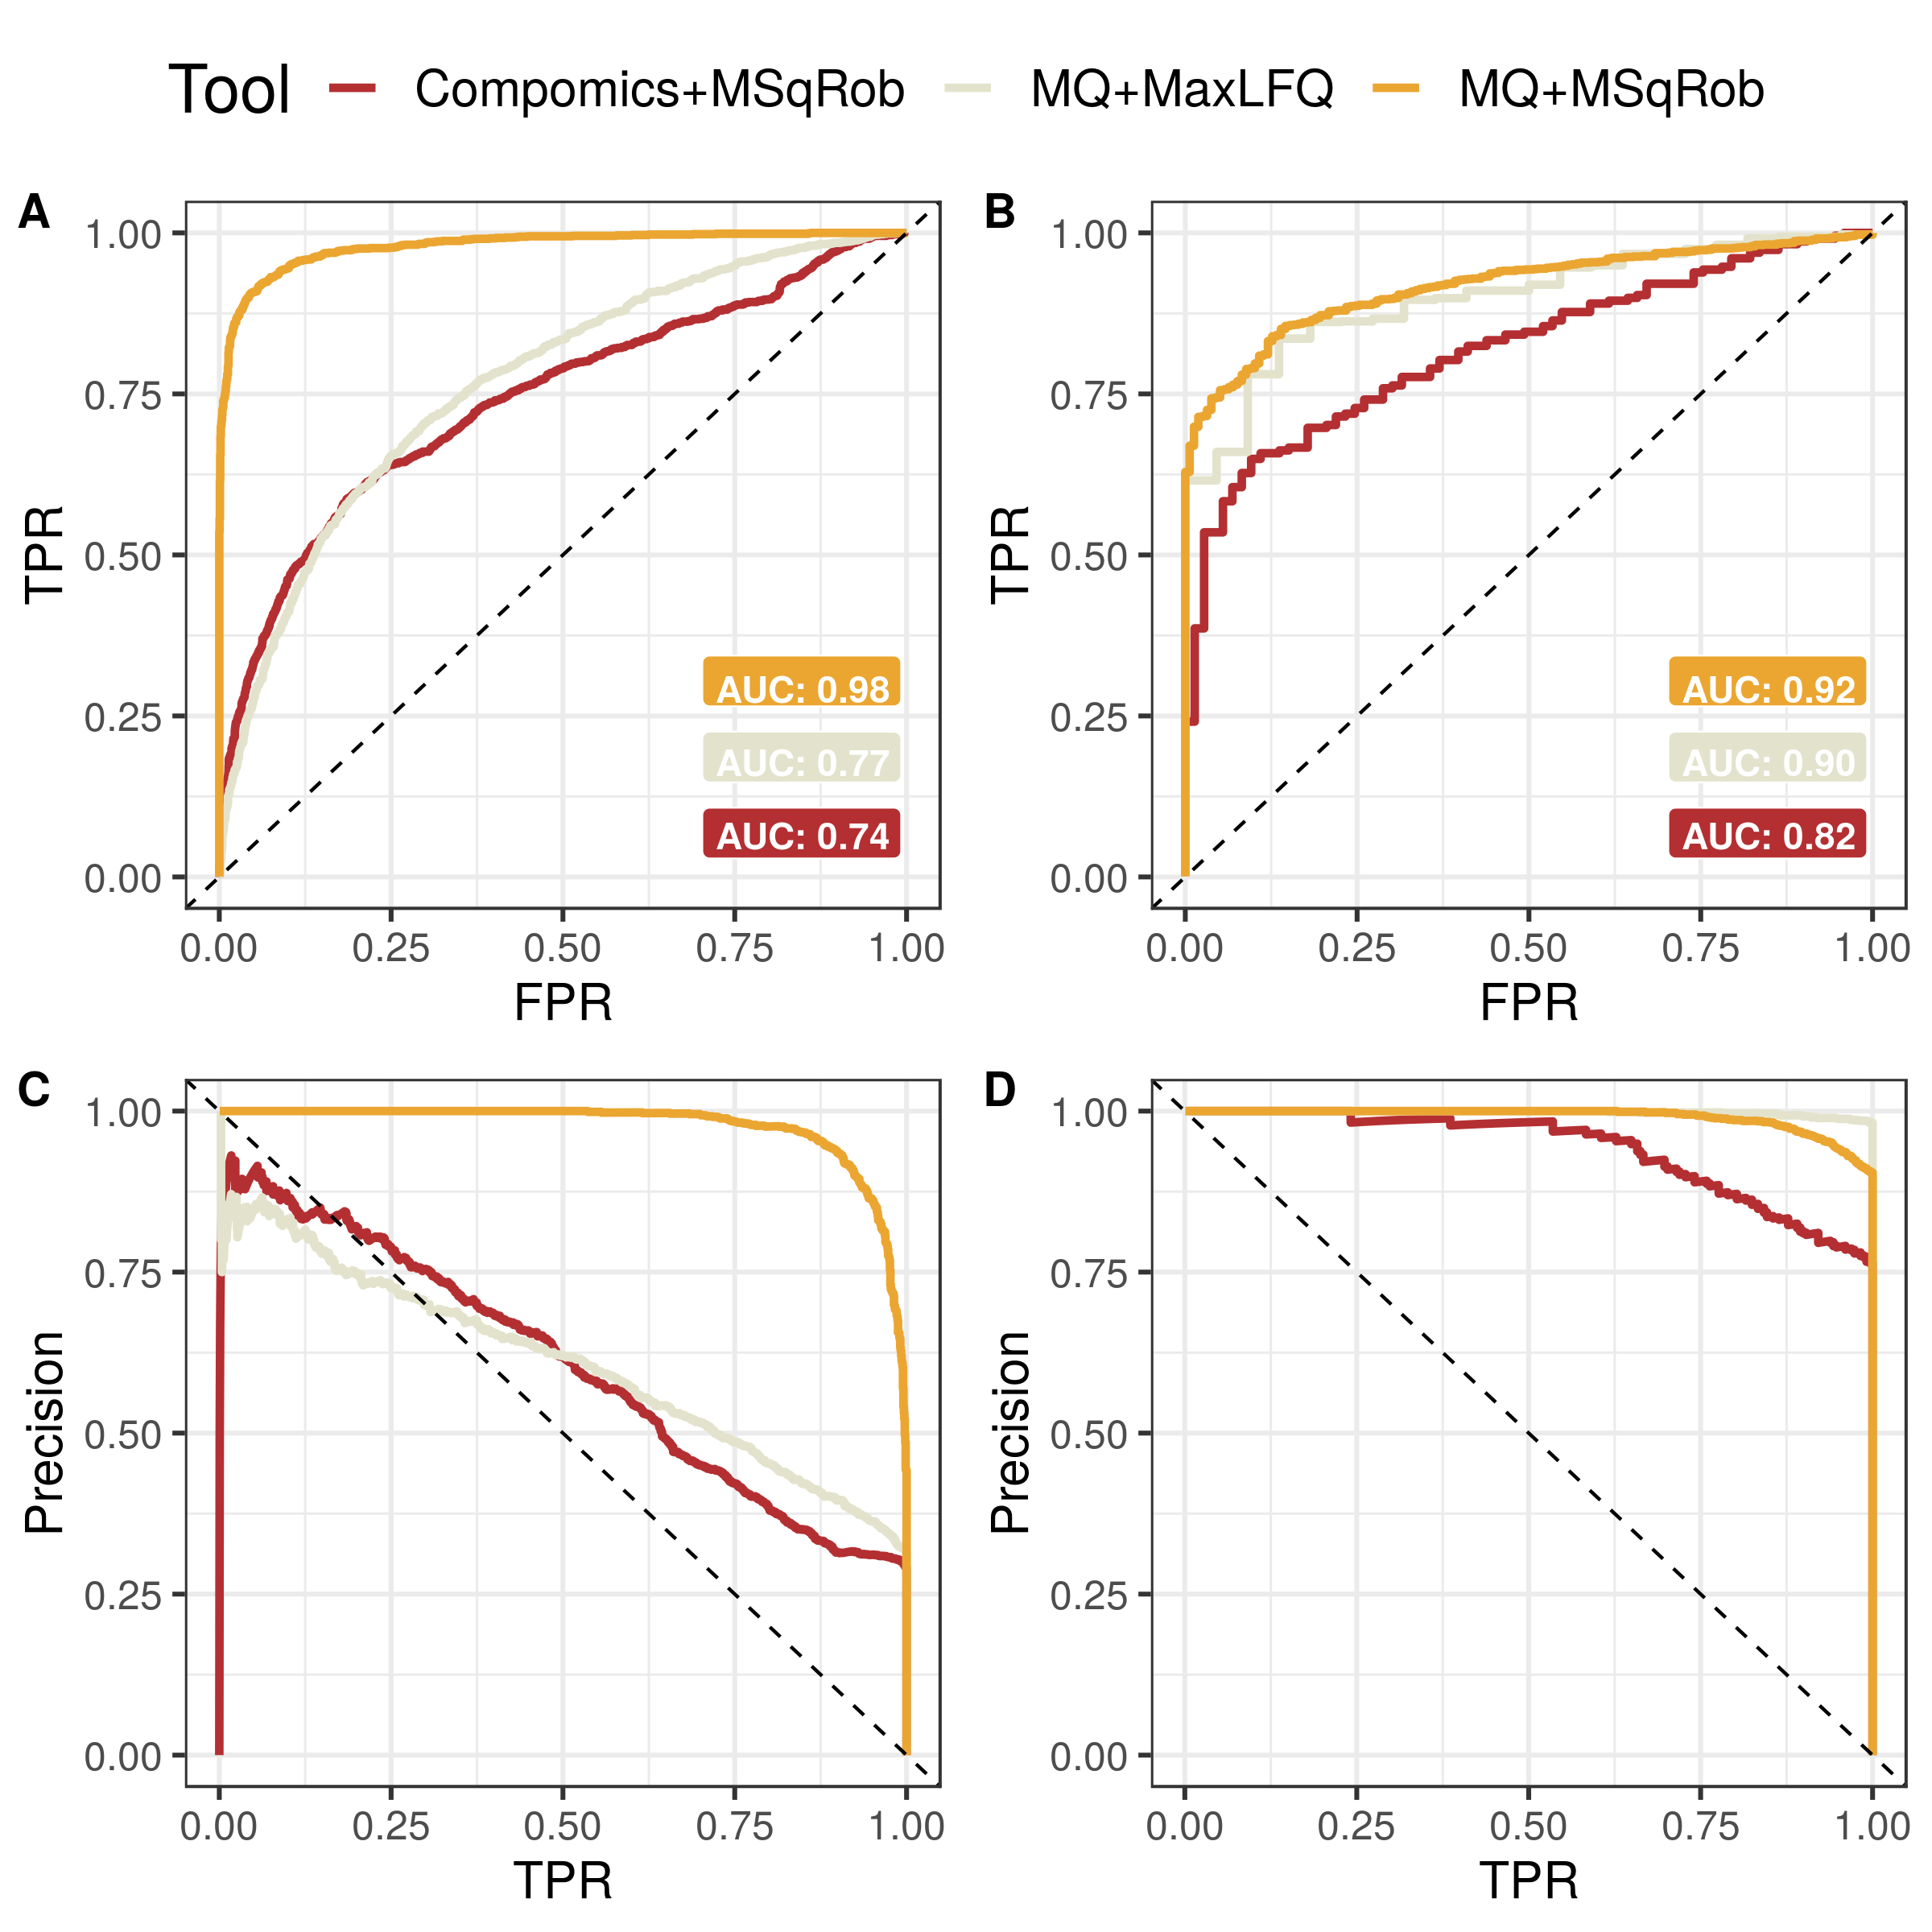
\includegraphics[width=\textwidth]{curves_plot}
\caption{ROC and PR curves displaying the behaviour of 3 different label-free quantification pipelines publicly available. \textbf{Comp+Rob} is the pipeline presented in the previous sections. \textbf{MQ+LFQ} consists a standard MaxQuant upstream analysis combined with its LFQ quantification engine. Finally, MQ+Rob blends MaxQuant upstream analysis with the MSqRob quantification engine. \textbf{A, B} ROC curve produced by the three algorithms with no \ac{log2FC} filter, and keeping proteins with \ac{log2FC} greater than 1, respectively. \textbf{C, D} PR curve produced by the three algorithms with no \ac{log2FC} filter, and keeping proteins with \ac{log2FC} greater than 1, respectively.}
\label{fig:roc_curves}
\end{figure}


Some of the most frequent evaluations of the performance of a binary classiffier are Receiver Operating Characteristic (ROC) and Precision-Recall (PR) curves \cite{Bradley1997}, which demonstrate the performance of the algorithm at different cutoff values of a predictor variable. Together, they show the False Positive Rate (FPR), the True Positive Rate (TPR) or recall, and the precision exhibited by the algorithm.




In the present problem, they can be used to show how good the \textit{q-val} associated to a protein group is at separating the two proteomes. Thus, \textit{E. coli} proteins are treated as positives, and those from \textit{Homo sapiens} are treated as negatives. Moreover, a filter based on the \ac{log2FC} can be applied to enrich the data in positives and facilitate the classification task.
In order to compare the results of the here presented pipeline (Comp+Rob) with those achieved by other available tools, the analysis was repeated using the data processing implemented in MaxQuant \cite{Cox2008} at different steps. The pipeline combining MaxQuant and MaxLFQ (MQ+LFQ) was fully carried out using the MaxQuant suite, whereas the combination of MaxQuant and MSqRob (MQ+Rob) used MaxQuant up to the fraction normalization step.

The result of this analysis is shown in figure \ref{fig:roc_curves}. Remarkably, Comp+Rob achieved similar results to those resulting from MQ+LFQ. Nonetheless, the latter performed clearly better when the \ac{log2FC} filter was applied, indicating that a combined fold change and q-value criteria is best for declaring proteins as differentially abundant. In all cases MQ+Rob was as good as MQ+LFQ, if not much better.


\begin{figure}[H]
\centering
\begin{subfigure}{.40\textwidth}
\caption*{A}
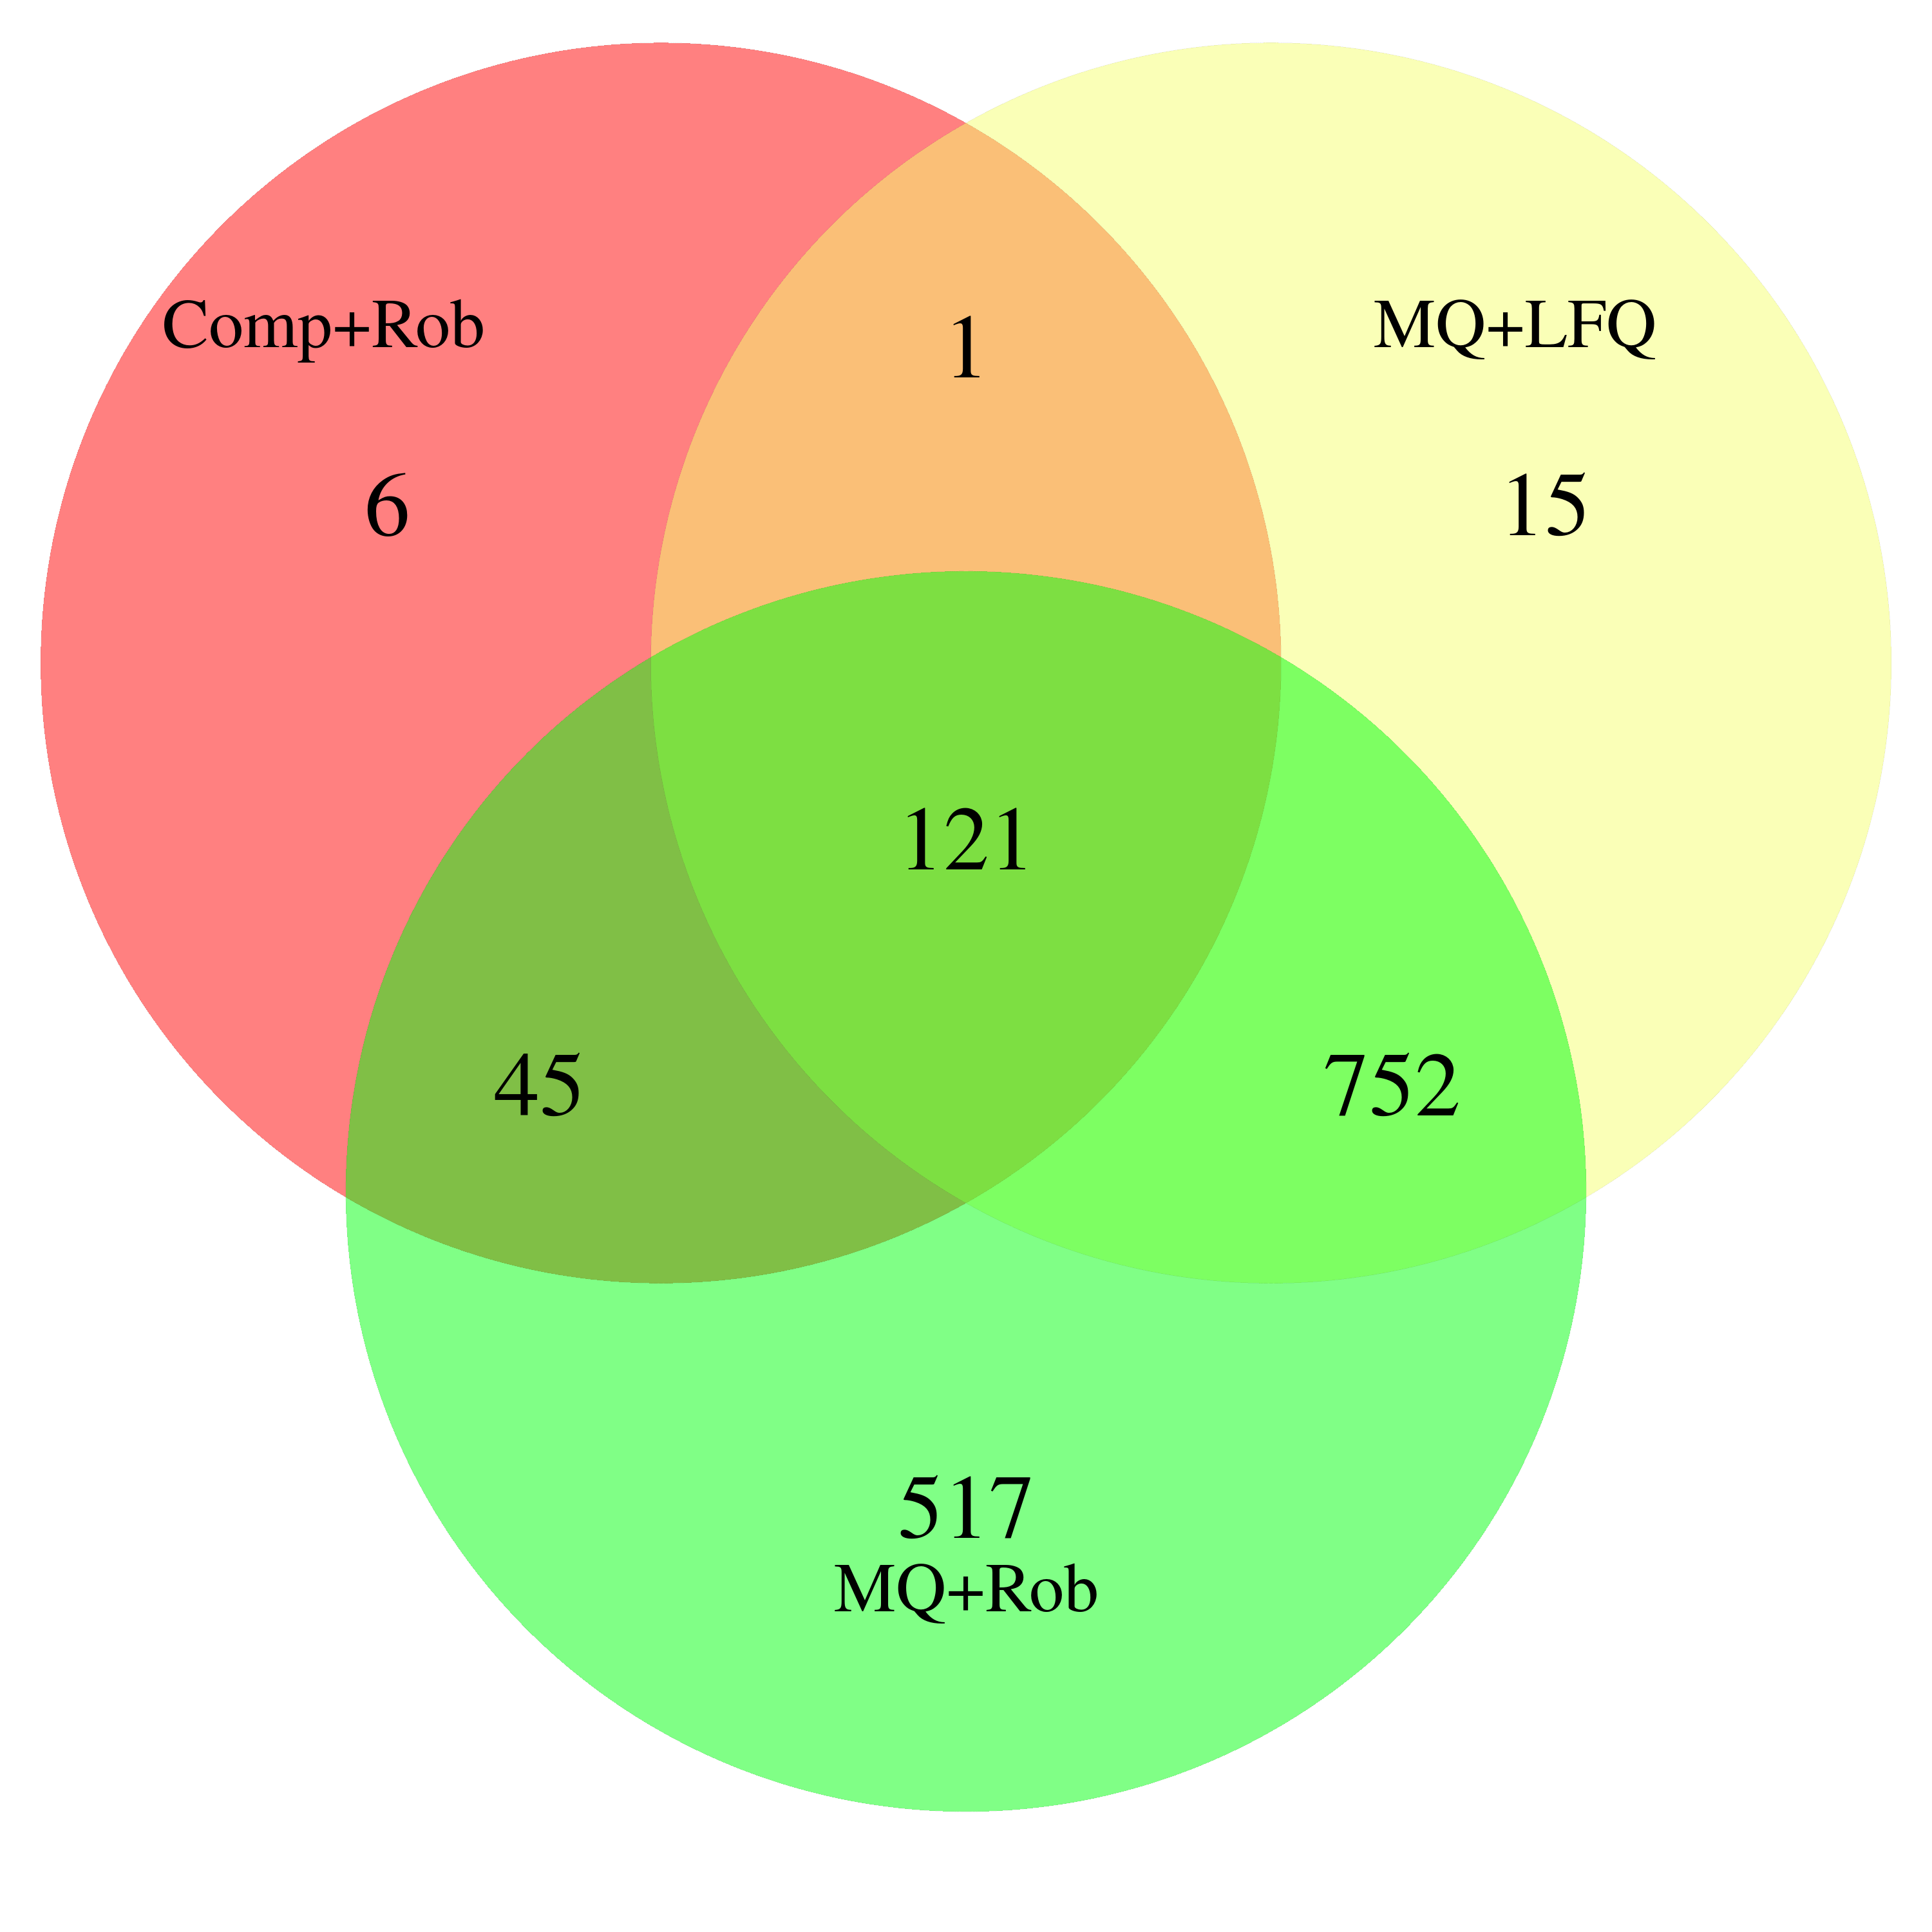
\includegraphics[width=.9\textwidth]{vennDiagram}
\end{subfigure}
\begin{subfigure}{.52\textwidth}
\caption*{B}
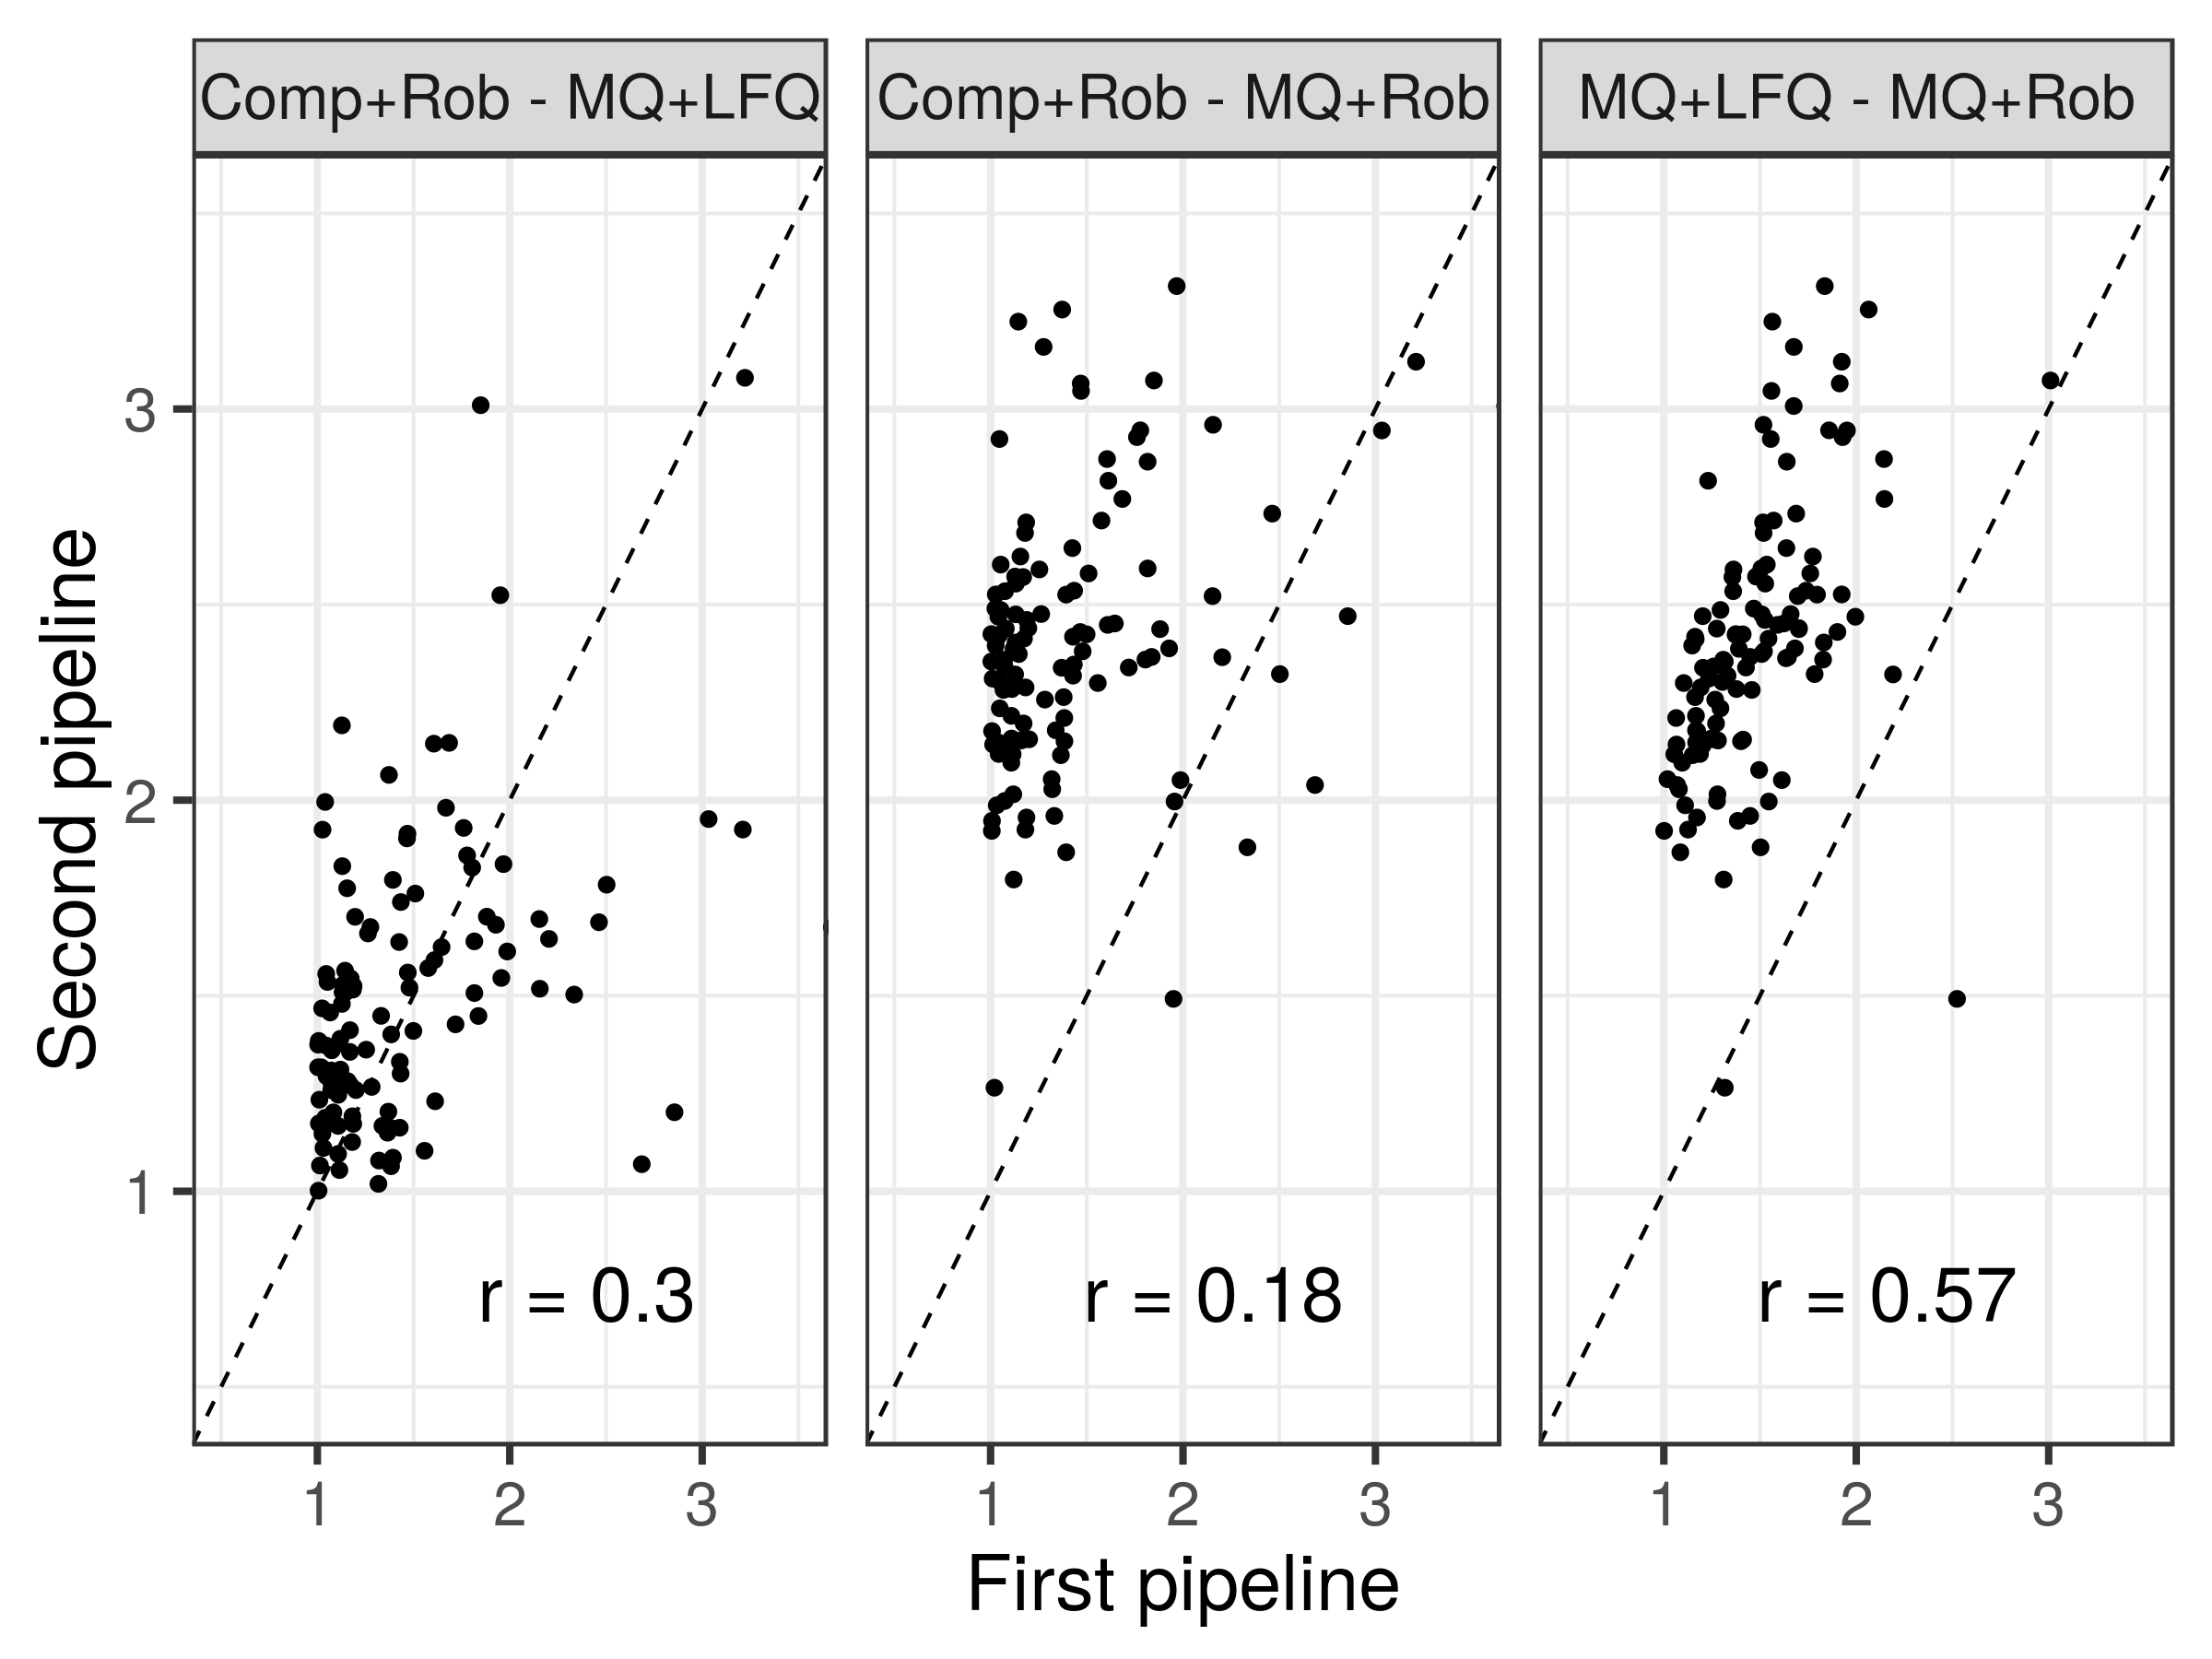
\includegraphics[width=.95\textwidth]{correlation_plot}
\end{subfigure}
\caption{Agreement between the different pipelines. \textbf{A} The Venn diagram displays the number of \textit{E. coli} proteins found to be differentially abundant by each pipeline. \textbf{B} The log2FC estimated in all three pipelines for the 121 shared proteins is plotted by pairs to evaluate their correlation.}
\label{fig:venn_cor}
\end{figure}


In order to visualize the level of agreement of the pipelines for the assignment of differentially abundant proteins, a Venn diagram was constructed (see figure \ref{fig:venn_cor} A). Venn diagrams provide a straightforward visualization of the overlap of several ensembles of proteins. The scrutiny of the counts reveals a high degree of agreement, with most proteins detected by Comp+Rob or MQ+LFQ being detectd by MQ+Rob too. Remarkably, 517 proteins were detected by MQ+Rob alone, which further confirmed its resolving power. Analyzing the log2FC pairwise-correlation (see figure \ref{fig:venn_cor} B) reveals that the highest correlation was found between pipelines using MaxQuant as upstream spectra processor, as expected. Even though the observed correlation was low, the estimated log2FC was always greater than 1. The MQ+Rob pipeline systematically estimated \ac{log2FC} values greater than the other 2.


Additionally, the accuracy with which each program assigns a \ac{log2FC} estimate to each protein group, and how significantly different from the null value of 0 it was found to be, provides further insights on the pros and cons of each pipeline, as shown in figure \ref{fig:combined_plot}. This analysis confirmed that the pipeline providing the best separation between organisms was MQ+Rob.




\begin{figure}[H]
\centering
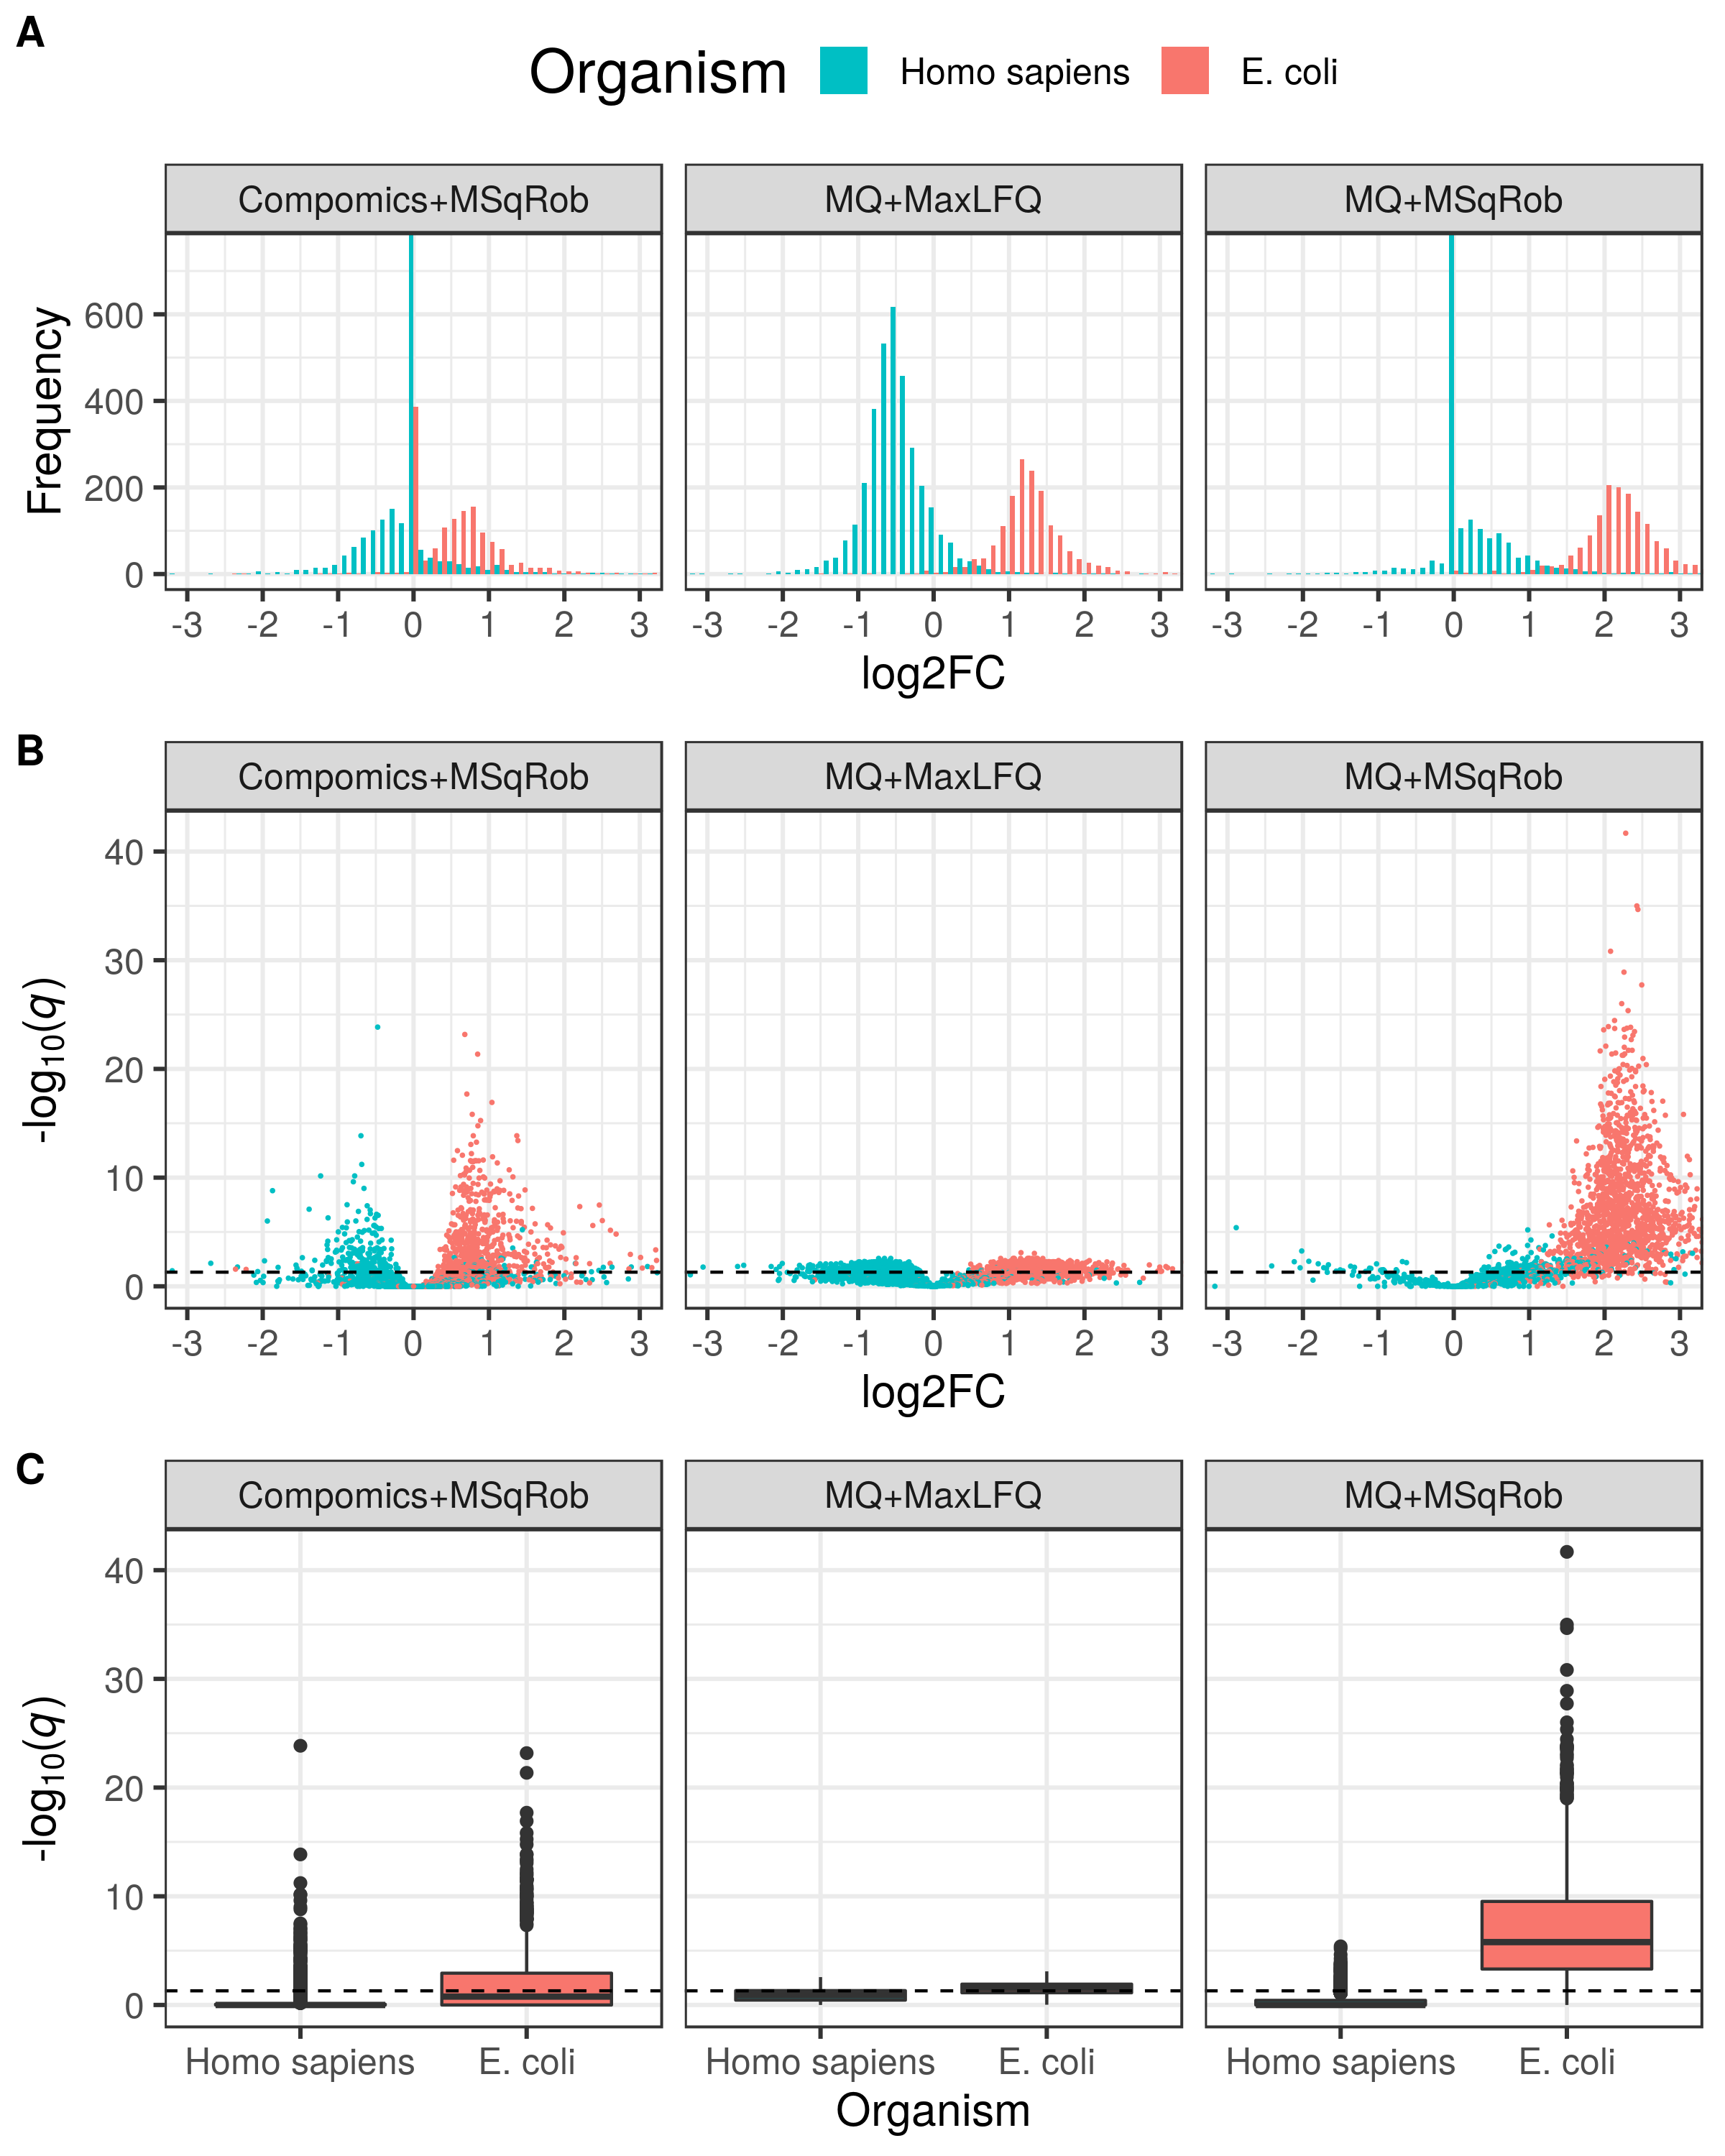
\includegraphics[width=\textwidth]{combined_plot}
\caption{Overview over the different pipelines\textquotesingle performance. Quantification results are segregated by the source organism. \textbf{A} Histogram of the \ac{log2FC} estimates. \textbf{B} Volcano plot, where every protein group is represented by a dot and the coordinates map to its \ac{log2FC} on x and the minus logarithm of the q-value on y. \textbf{C} Boxplots of the minus logarithm of the q-value distribution.}
\label{fig:combined_plot}
\end{figure}



\section{Discussion}

\subsection{Improvement of the PSM step}

The low attained matching rate manifests existing room for improvement in the currently available tools. As explained in section \ref{sec:search_engines}, it has been shown that the combined usage of multiple search engines can increase identifications, since the different statistical frameworks implemented in each of them compensate each other\textquotesingle s caveats. Only MS-GF+ was used in thi work for simplicity. Furthermore, \textit{de novo} search engines are available and supported by SearchGUI, and the latest developments in the field, like the IdentiPy engine \cite{Levitsky2018} are progressively incorporated to the tool \footnote{\href{https://github.com/compomics/peptide-shaker/issues/309}{https://github.com/compomics/peptide-shaker/issues/309}}. Their usage is predicted to improve identification rates and quality of the matches.

The most important reason why many spectra remain unidentified is the presence of post-translational modifications (\ac{PTM}s), which exponentially increase the search space, forcing most workflows to discard many of the peptides featuring a PTM. New approaches to the problem are emerging, mainly machine learning methods for the handling of unexpected modifications \cite{Gabriels}. Moreover, the prediction of \ac{MS2} peak intensities patterns from peptide sequences promises to increase the amount of evidence available during the PSM process, thus boosting correct identifications \cite{Kirik2018} \cite{Degroeve2013}.

Finally, the extremely low matching rates in the latter fractions translated to decreased contributions to the number of identifications. This indicated that decreasing the number of fractions would not have had a major impact in the experiment\textquotesingle s depth.

\subsection{Improvement of the feature extraction step}

While the apex intensity is a good estimate of the peptide abundance, other methods are available that could potentially provide more robust data, such as the area of the peak. This is the approach taken by the recently published tool RawQuant \cite{Kovalchik2018}, or the feature detection tool in the OpenMS pipeline \cite{Sturm2008}. Moreover, in order to fine tune the performance of the \ac{MBR} and Apex intensity extraction steps, several input arguments can be adapted to each dataset. These are the spectrometer\textquotesingle s \ac{m/z} resolution, the time window used during the apex search and whether or not to activate outlier filtering and what weights to use.

\subsection{Improvement of the quantification step}

The deployed relative quantification approach successfully manages to estimate the \ac{log2FC} of several of proteins in the dataset with high confidence. However, it was not found to be the best performing of the assayed pipelines in the benchmark dataset. Several axes of improvement are clear from the results.

\subsubsection{Management of sample fractionation}

Sample fractionation allows for a deeper analysis of the peptide mix, which in turn leads to increased identifications and an increased amount of data to be analyzed. However, it psimultaneously provides an extra random effect that difficults quantification if not handled properly.

The way the MaxLFQ engine solves the problem is by aggregating the data from the same sample across fractions using a ponderated average. One normalizing weight is determined for every sample via the \textit{Levenberg-Marquant minimisation of the overall proteome variation} $H(N)$ as defined in \cite{Cox2014}. A custom implementation was written in Python using the scipy module, but the results were not satisfactory.

MSqRob treats the fractions as a random effect, as explained in section \ref{subsec:quantification}. As a consequence, the statistical model in MSqRob can be overwhelmed by the inconsistency resulting from a 24-plex sample fractionation, leading to null \ac{log2FC} estimates for many \textit2{E. coli} proteins. This is clearly manifested in figure \ref{fig:combined_plot} as the bins at \ac{log2FC} of 0, which represent protein groups for which MSqRob did not find enough evidence to discard the null hypothesis. While no \textit{E. coli} proteins fell in this category in the MQ-MSqRob pipeline, many did in the Comp+Rob, proving room for improvement in this aspect.

In any case, the way sample fractionation is handled should depend upon the fractionation method. For example, membrane fractionation can be exploited when working with membrane proteins \cite{Marmagne2006}.

To sum up, the presently implemented fraction handling is correct and provides good results, but fine-tuning of the pipeline at this step is expected to improve the results of the quantification. Thanks to the open-source nature of the software, this is indeed possible.


%which is defined according to the following expressions:
%
%\begin{equation}
%I_{P,A}(\text{N}) = \sum\limits_{j=1}^{k}{\text{N}_{A,j} \times \text{XIC}_{P,A,j}}
%\end{equation}
%
%where $\text{N}_{A,j}$ stands for the normalization coefficient for sample $A$ and fraction $j$, and $\text{XIC}_{P,A,j}$ stands for the extracted ion current in the same sample and fraction for peptide P. The sum runs over all k fractions.
%
%\begin{equation}
%H_P(N) = \sum\limits_{A,B} \abs{\log(\frac{I_{P,A}(N)}{I_{P,B}(N)})}^2
%\end{equation}
%
%\begin{equation}
%H(N) = \sum\limits_{p} H_p(N) 
%\end{equation}
%
%where the pair $A$ and $B$ is any of the sample pairs where peptide $P$ is detected. The overall proteome variation is 


\subsubsection{The pitfalls of mass spectrometry}

The application of mass spectrometry to proteomics is a very hot topic in research, driving innovations in the way the different components of the spectrometer work. One recent example is the development of the timsTOF\texttrademark\xspace Pro (Trapped Ion Mobility Spectrometry-Time Of Flight) system by Bruker, which supports PASEF (Parallel Accumulation and SErial Fragmentation) spectrometry \footnote{\href{https://www.prnewswire.com/news-releases/bruker-launches-the-timstof-pro-mass-spectrometer-to-enable-the-revolutionary-pasef-method-for-next-generation-proteomics-300520791.html}{https://www.prnewswire.com/news-releases/bruker-launches-the-timstof-pro-mass-spectrometer-to-enable-the-revolutionary-pasef-method-for-next-generation-proteomics-300520791.html}}. This technology adds  an extra dimension peptide separation process, leading to cleaner spectra.
Notwithstanding, the developments also reveal the immature state of the technology. Slight inconsistencies in the protein extraction and digestion, bias in the peptide ionization, presence of unexpected PTMs, and detector saturation and insensitivity, remain as problems contributing to the eventual measurement variability characteristic of mass spectrometry \cite{Piehowski2013}. Thus, adequate cleaning of the peptide dataset, and care to ignore outliers is preeminent. Indeed, the input file for the MQ+LFQ consisted of a preprocessed file which removed the most problematic proteins \cite{Cox2014}, which explains why more than 500 extra proteins could be quantified when using MSqRob (see figure \ref{fig:venn_cor} A).

\subsubsection{Support for absolute quantification}

While relative quantification like that performed by MSqRob is enough to infer differential abundance of proteins across conditions, absolute quantification would provide an estimate of protein quantities that would support many other analyses, and facilitate comparison between datasets, in a way similar to what the normalised read counts in FPKM (Fragments Per Kilobase per Million Reads) does in transcriptomics. On the other hand, MaxLFQ provides absolute estimates, albeit less robust.

\subsubsection{Quantification of uncertainty}

All the quantification approaches enunciated until now make use of different frequentist approaches to the problem, that evaluate how significantly different the data are from what would be expected under a null hypothesis of a null ratio across the pair of conditions. Yet, it does not provide probabilistic interpretations of the uncertainty behind the estimate. The development of a Bayesian framework which endeavors at solving this issue is presented in chapter \ref{chap:model}.


\section{Conclusion}

An open-source, free, platform-agnostic and customisable label-free relative quantification pipeline assembling publicly available tools was presented in this work. The pipeline is capable of providing qualitative information on the protein composition of a sample using the latest proteomics search engines and validation software. Moreover, it can be extended to support more complex tasks, like \textit{De novo} search, or the study of \ac{PTM}s, thanks to its non-monolithic nature and usage of open-formats. Likewise, the openness of the data in all steps allows for quality control checks along the way. However, the comparison against other workflows shows the room for improvement in the quantification step when dealing with fractionated data, albeit deficiencies in this aspect should have no impact in non-fractionated datasets.

Either the pipeline developed in the presented chapter or those based on MaxQuant are ready to be deployed in a real environment and provide \ac{NZ} with useful insights on its proteomics data for free.